\documentclass[11pt, oneside]{amsart}   	% use "amsart" instead of "article" for AMSLaTeX format
\usepackage{geometry}                		% See geometry.pdf to learn the layout options. There are lots.
\geometry{letterpaper}                   		% ... or a4paper or a5paper or ... 
%\geometry{landscape}                		% Activate for rotated page geometry
%\usepackage[parfill]{parskip}    		% Activate to begin paragraphs with an empty line rather than an indent
\usepackage{graphicx}				% Use pdf, png, jpg, or eps§ with pdflatex; use eps in DVI mode
								% TeX will automatically convert eps --> pdf in pdflatex		
\usepackage{amssymb}
\usepackage[]{hyperref}
\usepackage{listings}

%----macros begin-----------------------------------------------------------------------------------
\usepackage{graphicx}
\usepackage{color}
\usepackage{xcolor}
\usepackage{amsfonts}
\usepackage{amsmath}
%\usepackage{amsthm}
%\usepackage[utf8]{inputenc}

%\renewenvironment{Shaded}{\pause\begin{snugshade}}{\end{snugshade}}
\def\twocolumns#1#2{\begin{columns}
\begin{column}{0.5\linewidth}#1\end{column}
\begin{column}{0.5\linewidth}#2\end{column}
\end{columns}}
\def\mytwocolumns#1#2#3#4{\begin{columns}
\begin{column}{#1\linewidth}#2\end{column}
\begin{column}{#3\linewidth}#4\end{column}
\end{columns}}
\def\mythreecolumns#1#2#3#4#5#6{\begin{columns}
\begin{column}{#1\linewidth}#2\end{column}
\begin{column}{#3\linewidth}#4\end{column}
\begin{column}{#5\linewidth}#6\end{column}
\end{columns}}
\def\threecolumns#1#2#3{\begin{columns}
\begin{column}{0.33\linewidth}#1\end{column}
\begin{column}{0.33\linewidth}#2\end{column}
\begin{column}{0.33\linewidth}#3\end{column}
\end{columns}}
\def\fourcolumns#1#2#3#4{\begin{columns}%
\begin{column}{0.25\linewidth}#1\end{column}%
\begin{column}{0.25\linewidth}#2\end{column}%
\begin{column}{0.25\linewidth}#3\end{column}%
\begin{column}{0.25\linewidth}#4\end{column}%
\end{columns}}

\def\conv{\mbox{\textrm{conv}\,}}
\def\aff{\mbox{\textrm{aff}\,}}
\def\E{\mathbb{E}}
\def\R{\mathbb{R}}
\def\Z{\mathbb{Z}}
\def\N{\mathbb{N}}
\def\v#1{{\bf #1}}
\def\p#1{{\bf #1}}
\def\T#1{{\bf #1}}
\def\vet#1{{\left(\begin{array}{cccccccccccccccccccc}#1\end{array}\right)}}
\def\mat#1{{\left(\begin{array}{cccccccccccccccccccccccccccc}#1\end{array}\right)}}

\def\lin{\mbox{\rm lin}\,}
\def\aff{\mbox{\rm aff}\,}
\def\pos{\mbox{\rm pos}\,}
\def\cone{\mbox{\rm cone}\,}
\def\conv{\mbox{\rm conv}\,}
\newcommand{\homog}[0]{\mbox{\rm homog}\,}
\newcommand{\relint}[0]{\mbox{\rm relint}\,}

%----macros end-----------------------------------------------------------------------------------


\title[Addendum]{Addendum}
\author{to ``Topological computing of arrangements with (co)chains''}
\date{\today}							% Activate to display a given date or no date

\begin{document}
\maketitle
\thispagestyle{empty}
%\section{}
%\subsection{}


\begin{figure}[htbp] %  figure placement: here, top, bottom, or page
   \centering
   %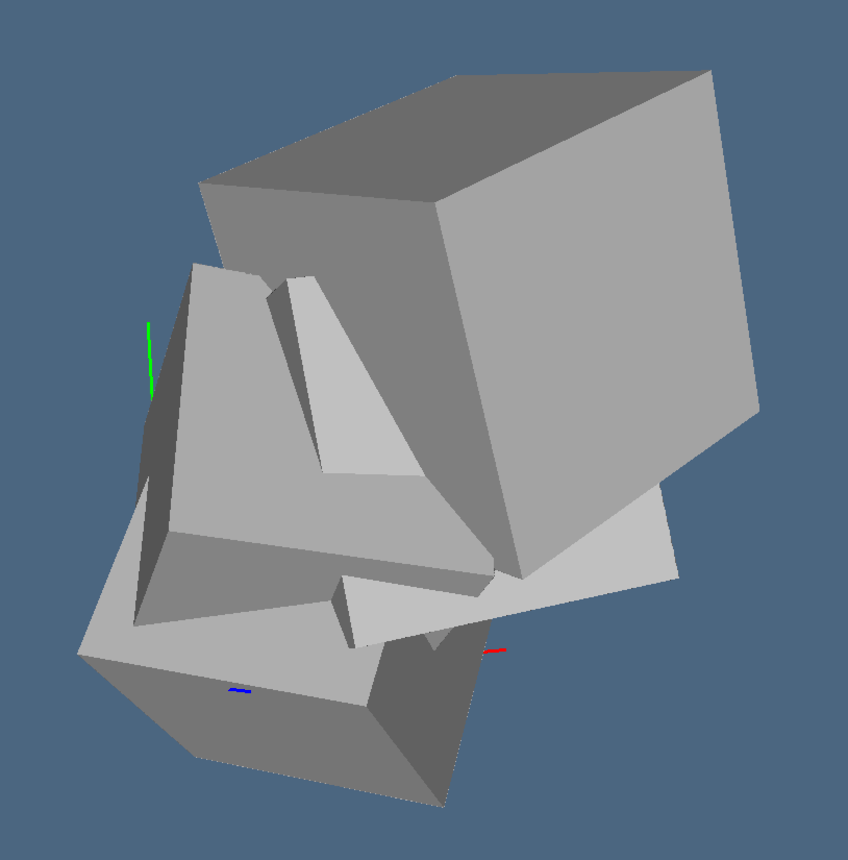
\includegraphics[width=0.20\textwidth]{img/1.pdf}%
   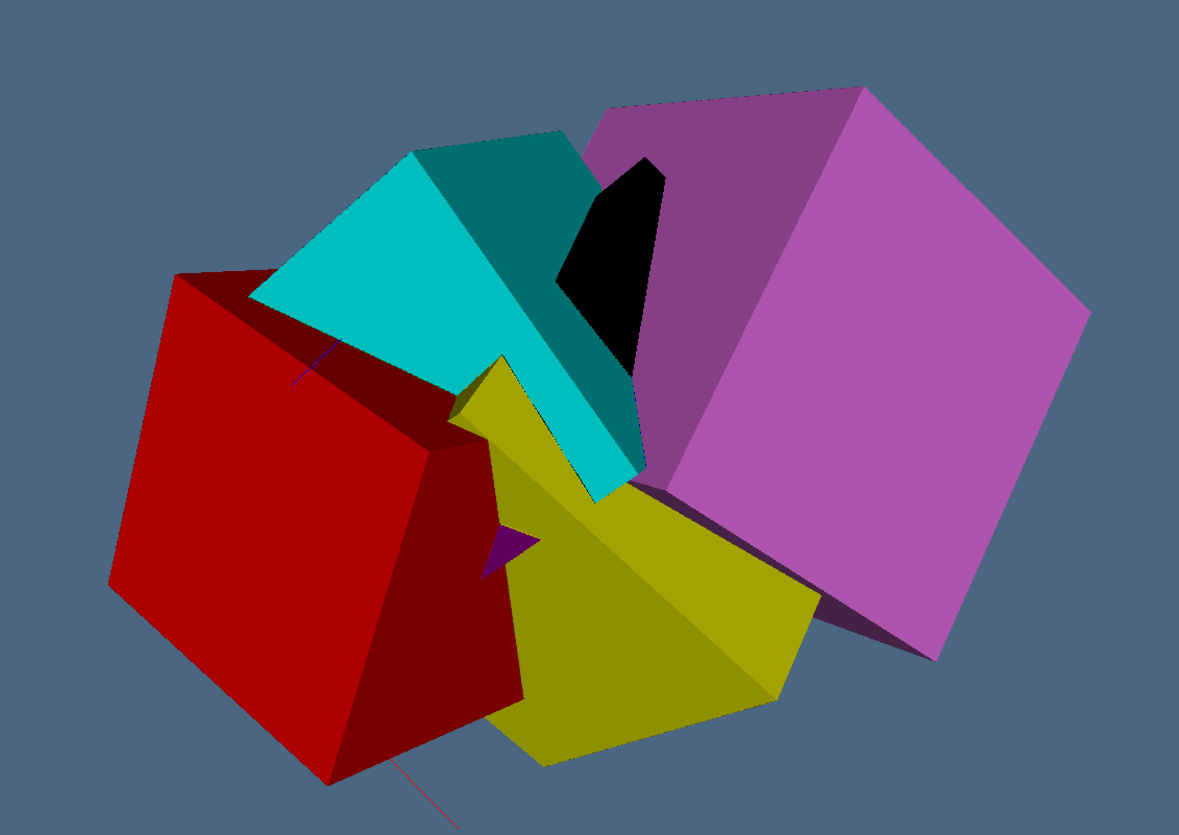
\includegraphics[width=0.50\textwidth]{img/32.pdf}%
   %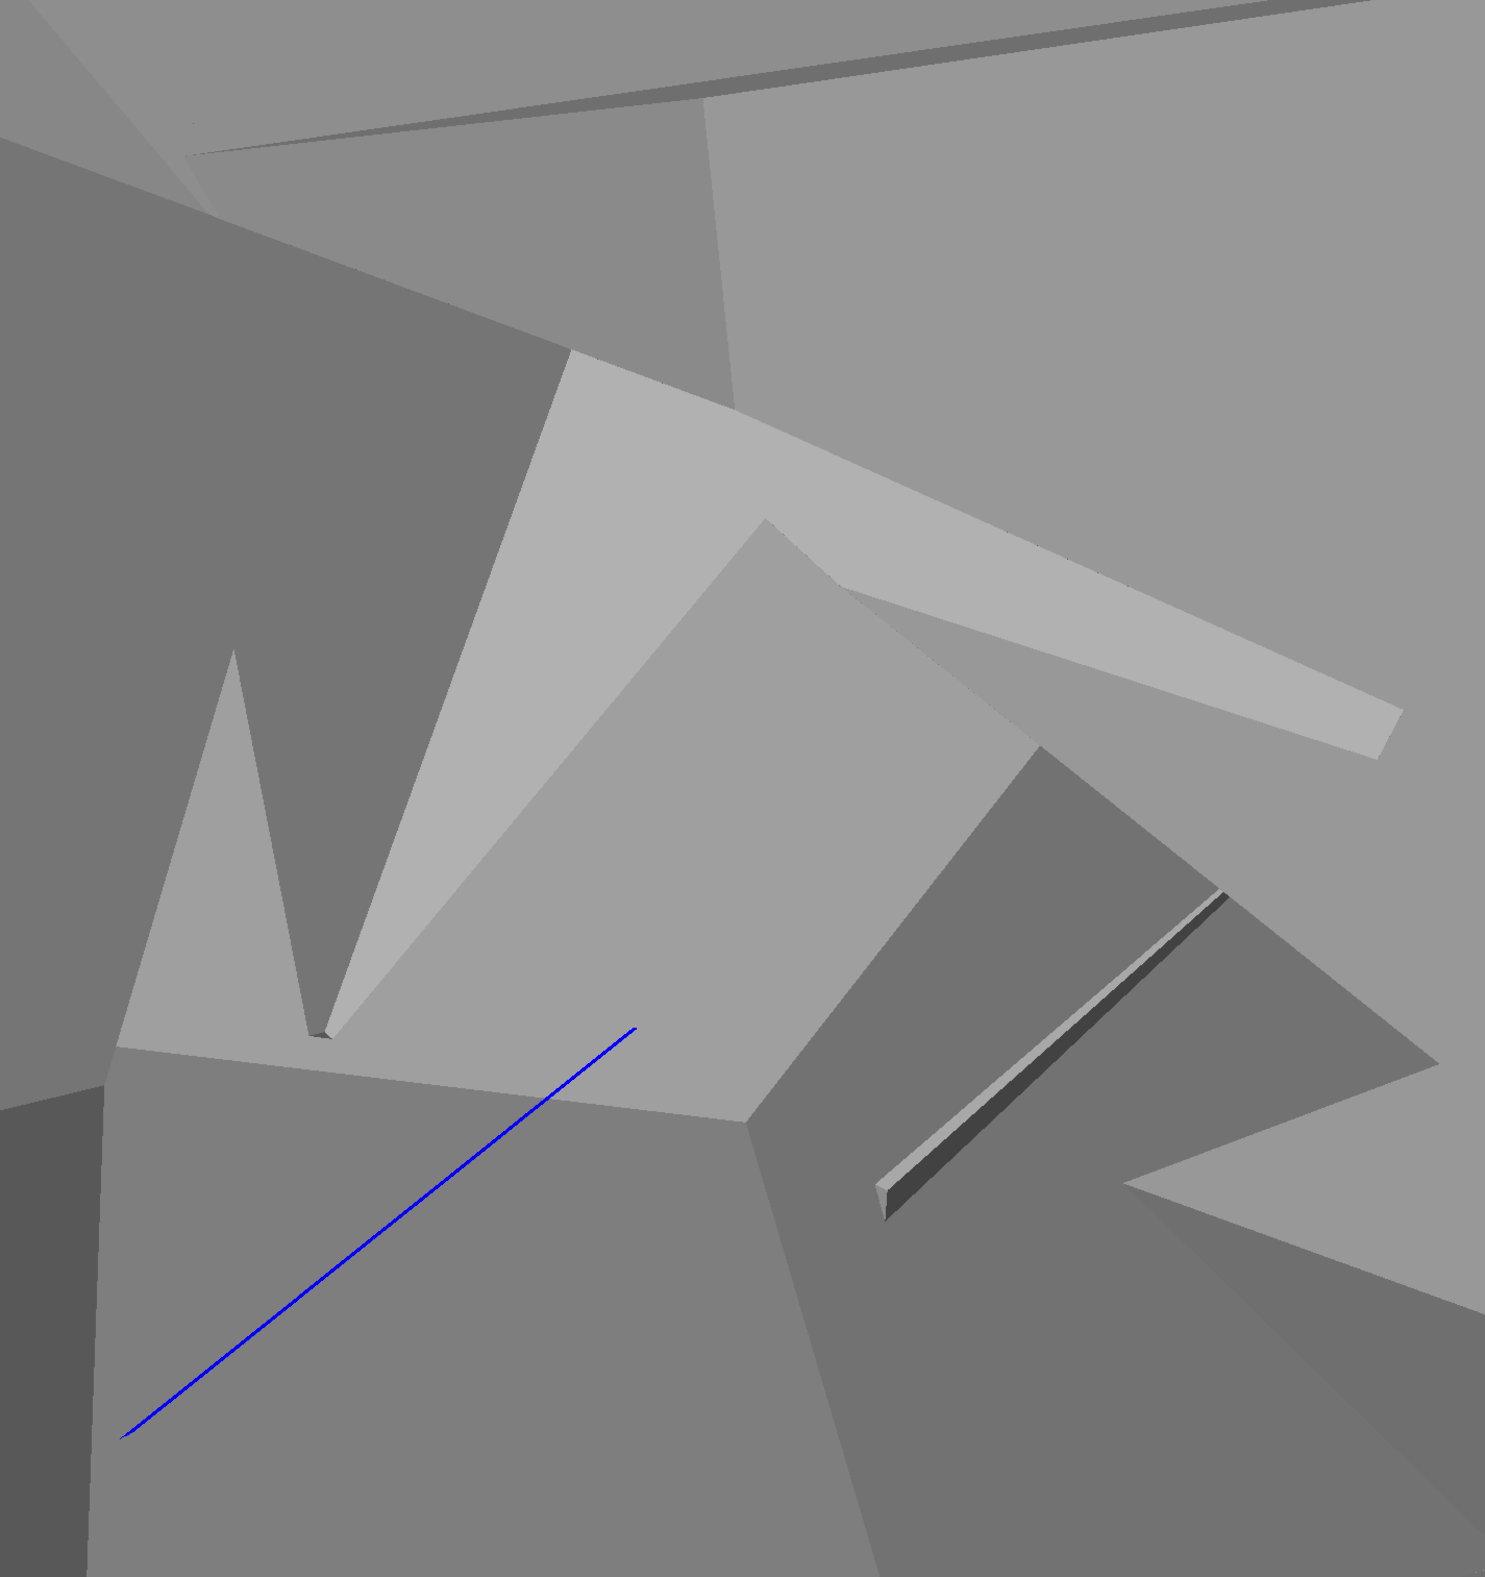
\includegraphics[width=0.19\textwidth]{img/31.pdf}%
   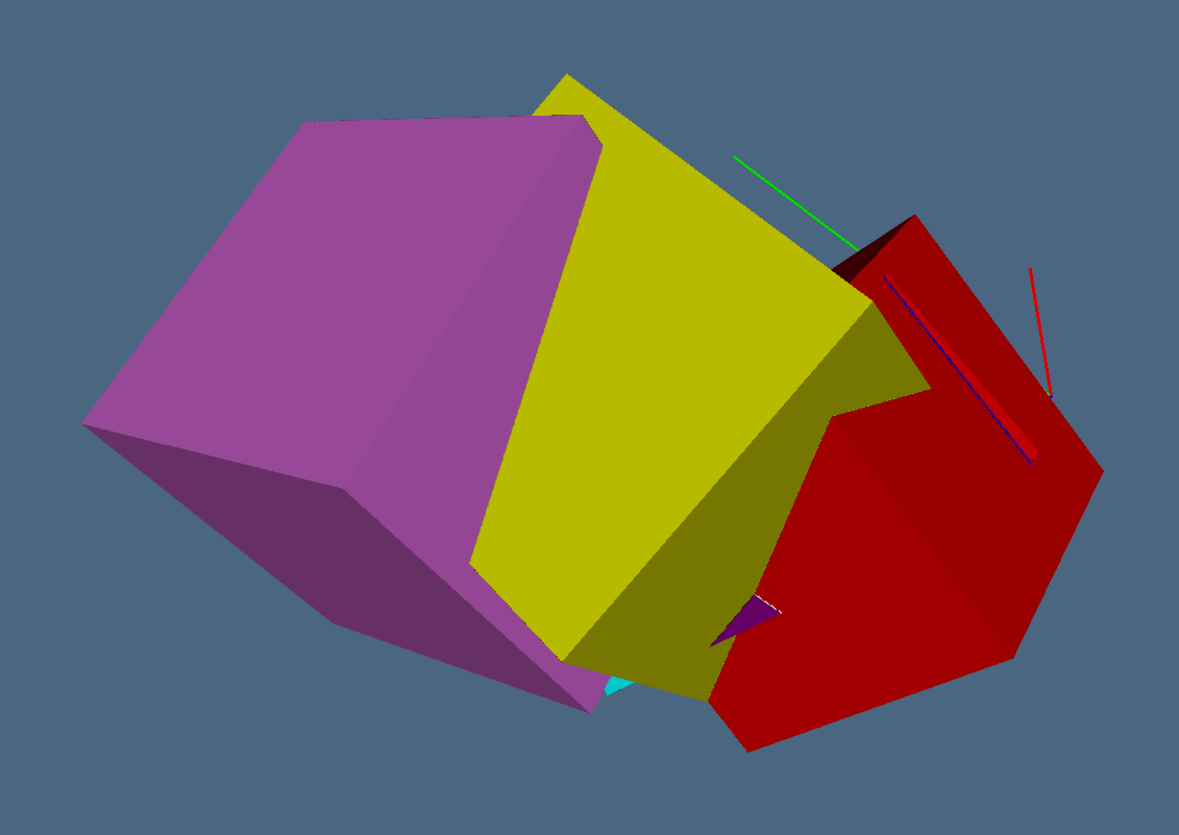
\includegraphics[width=0.50\textwidth]{img/34.pdf}%
   %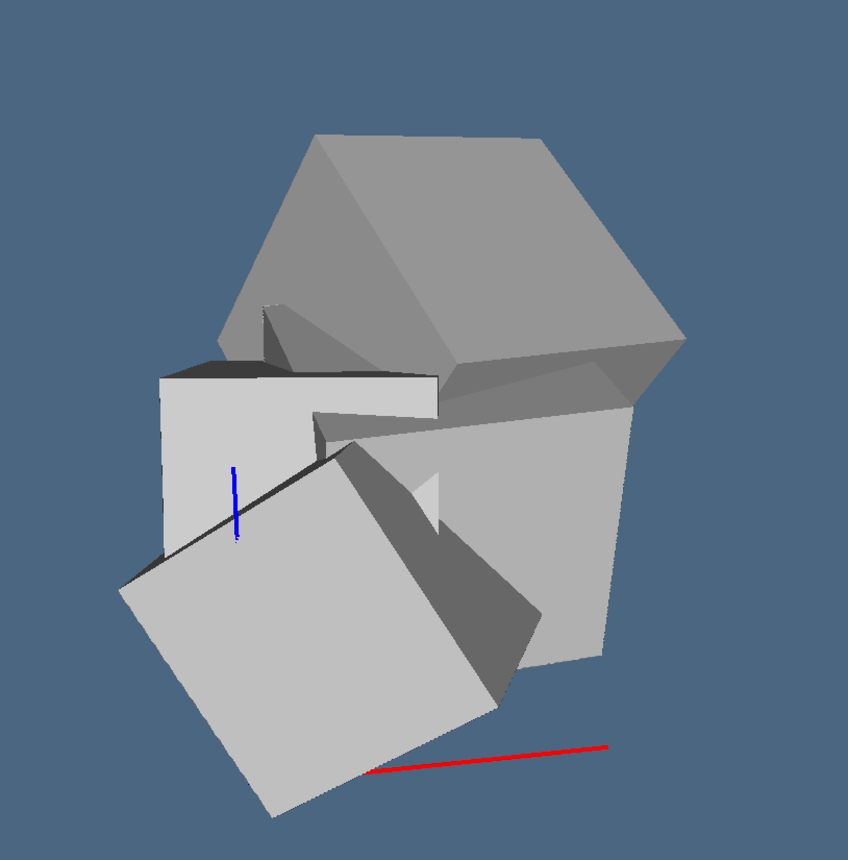
\includegraphics[width=0.20\textwidth]{img/30.pdf}%
   
   \caption{Two images of the biggest 3-cell, whose outer 2-boundary coincides with the (reversed) 2-boundary of the outer space (outer 3-cell).}
   \label{fig:input}
\end{figure}

\nonstopmode


\begin{quote}
Archimedes to Eratosthenes greeting. ... certain things first became clear to me by a mechanical method, although they had to be demonstrated by geometry afterwards because their investigation by the said method did not furnish an actual demonstration. But it is of course easier, when we have previously acquired by the method, some knowledge of the questions, to supply the proof, than it is to find it without any previous knowledge.

\flushright \emph{The Method}
\end{quote}


%===============================================================================
\section{Introduction}
%===============================================================================
The aims of this short essay are:  (a) to give an example of the computational techniques introduced with the paper ``Topological computing of arrangements with (co)chains''~\cite{TSAS}, submitted about two years ago to ACM Transactions on Spatial Algorithms and Systems (TSAS), and (b) to produce some  measures providing a benchmark of this approach. 
\newpage

We intend to illustrate here the input and the output data generated by our open-source  implementation\footnote{{\footnotesize
\href{https://github.com/cvdlab/LinearAlgebraicRepresentation.jl/tree/julia-1.0}{See our \texttt{Github.com} repository},
}}, when applied to a small collection of closed polyhedral surfaces, so producing the \emph{arrangement} (partition) of 3D space, described by the matrices of linear operators $\delta_0, \delta_1, \delta_2$ and their transposed operators $\partial_1, \partial_3, \partial_2$, which go up and down, respectively, between linear chain spaces $C_0, C_1, C_2$ generated by the 3D partition.

For problem statement, motivation, definitions, discussions, algorithms, applications, and further examples, the reader is  referred to~\cite{TSAS}.
We discuss in the present paper the Julia's script solving the arrangement problem and the output generated, starting from five randomly oriented and dimensioned cubes around the origin, which are shown in Figure~\ref{fig:input}. Finally we compare the amount of data produced by this approach with the more crude raw format of graphics applications, i.e.~the boundary triangle mesh of generated 3-cells. 



%===============================================================================
\section{Computation of 3D arrangement example}
%===============================================================================

\subsection{Partition into solid cells}
%-------------------------------------------------------------------------------

A \emph{chain complex} is a short exact sequence of graded linear spaces \(C_p\) of (co)chains, with linear
boundary/coboundary maps \(\partial_p\) and
\(\delta_p=\partial_{p+1}^\top\): 
\[ 
C_\bullet = (C_p, \partial_p) := 
C_3 \ 
\substack{
\delta_2 \\
\longleftarrow \\[-1mm]
\longrightarrow \\
\partial_3 
}
\ C_2 \ 
\substack{
\delta_1 \\
\longleftarrow \\[-1mm]
\longrightarrow \\
\partial_2 
}
\ C_1 \ 
\substack{
\delta_0 \\
\longleftarrow \\[-1mm]
\longrightarrow \\
\partial_1 
}
\ C_0 .
\] 

The cells of a space partition are one-to-one with the basis elements of chain spaces. The chain maps ($\partial_p$ or $\delta_p$) fully describe the topology of the cellular arrangement.

\begin{figure}[htbp] %  figure placement: here, top, bottom, or page
   \centering
   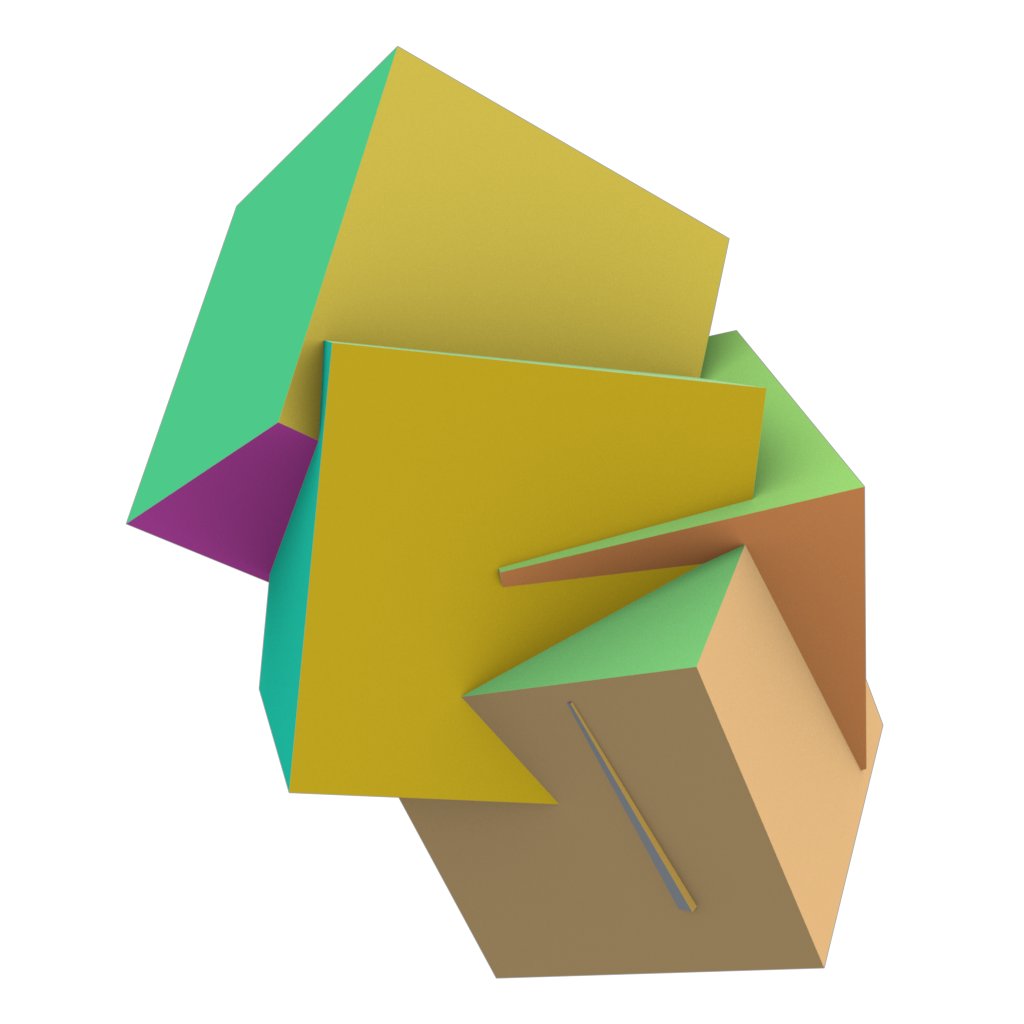
\includegraphics[width=0.5\textwidth]{images/0001.png}%
   \caption{The boundary of the whole assembly, which can be also denoted as the boundary of the outer (or exterior) 3-cell. This image and the following images of single 3-cells were rendered with Autodesk Maya.
   }
   \label{fig:example}
\end{figure}

The set of manifold 3-cells of the 3D arrangement produced by the surfaces in Figure~\ref{fig:input} is shown in Figure~\ref{fig:3-cells}. It is worthwhile to note that such solid cells may be non-convex and non-contractible, i.e.,~non simply connected. Such properties extend to their 2-cell faces. 

It may be interesting to notice also that cells may have different topological genuses, i.e.,~any number of holes and tunnels. 
\begin{figure}[htbp] %  figure placement: here, top, bottom, or page
%   \centering
   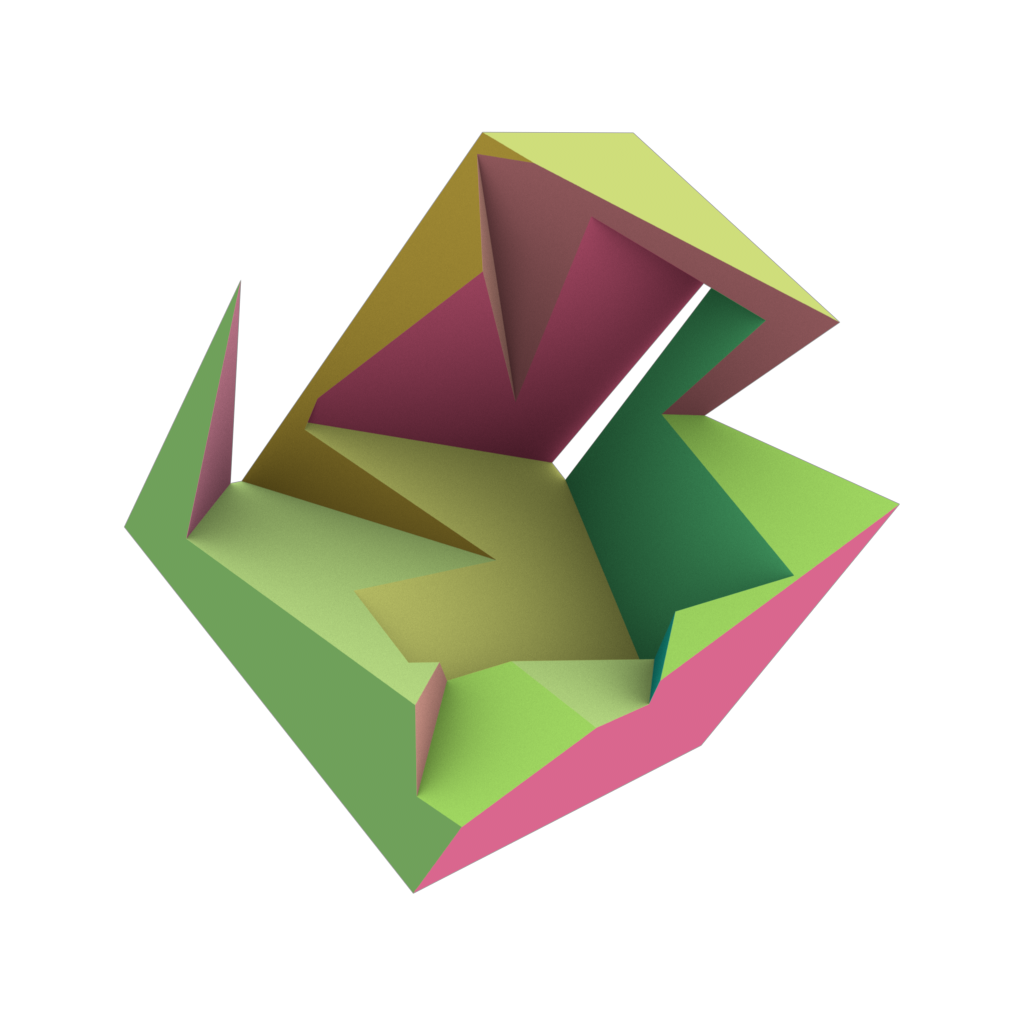
\includegraphics[width=0.26\textwidth]{images/0002.png}\hspace{-9mm}%
   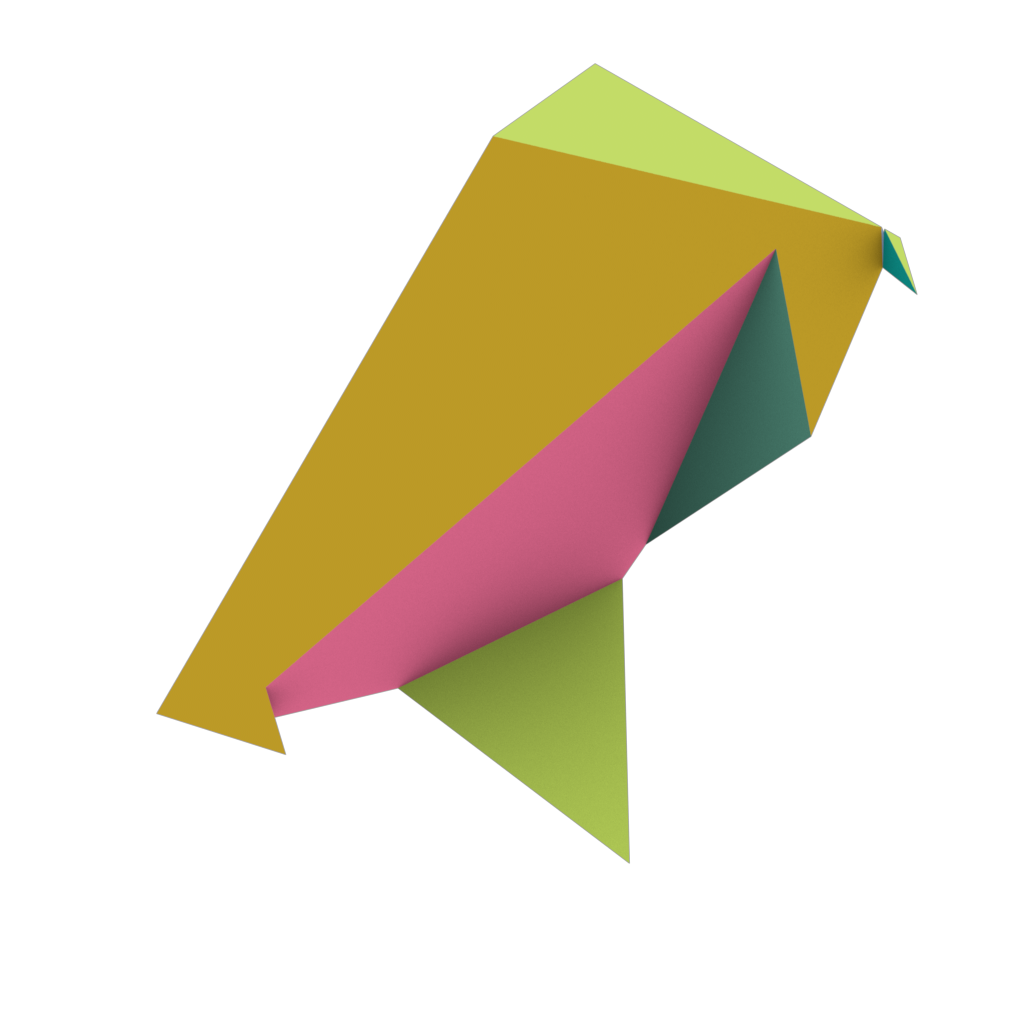
\includegraphics[width=0.22\textwidth]{images/0003.png}\hspace{-7mm}%
   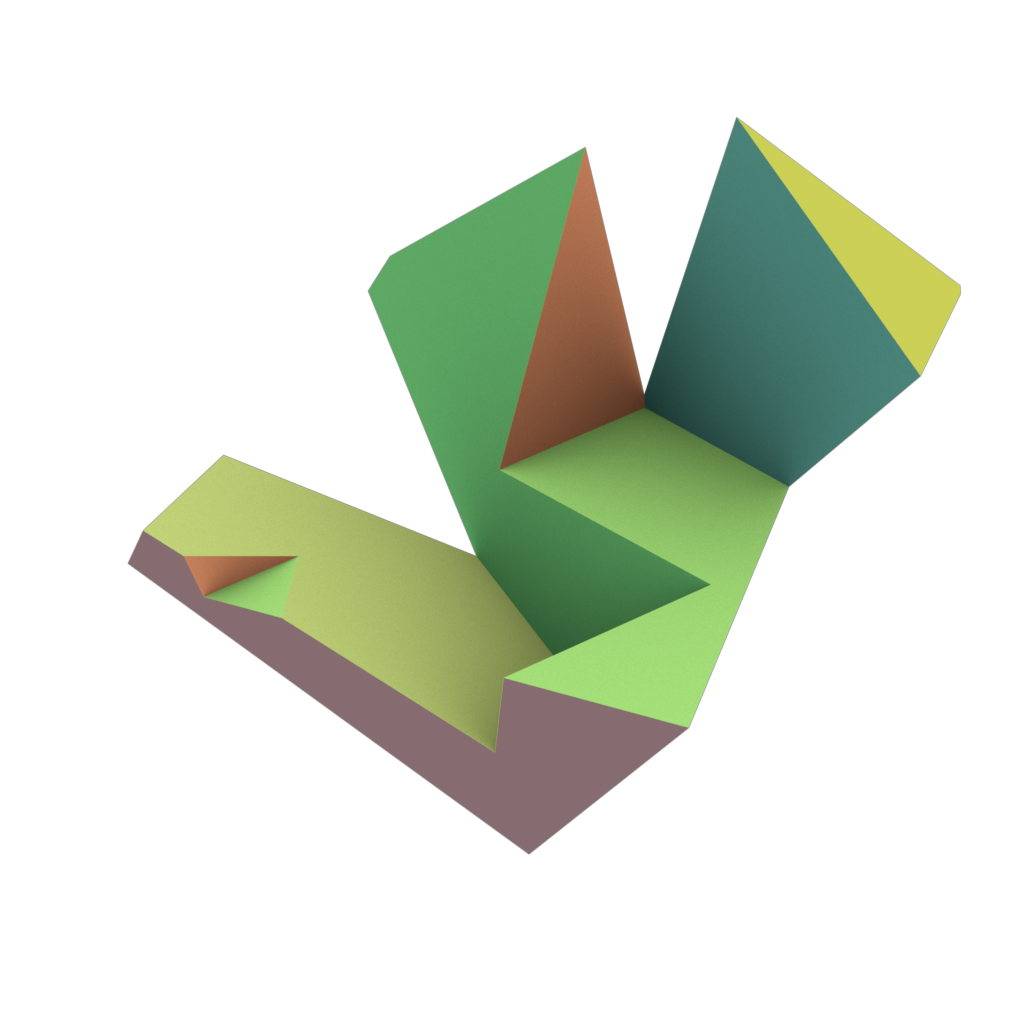
\includegraphics[width=0.24\textwidth]{images/0004.png}\hspace{-7mm}%
   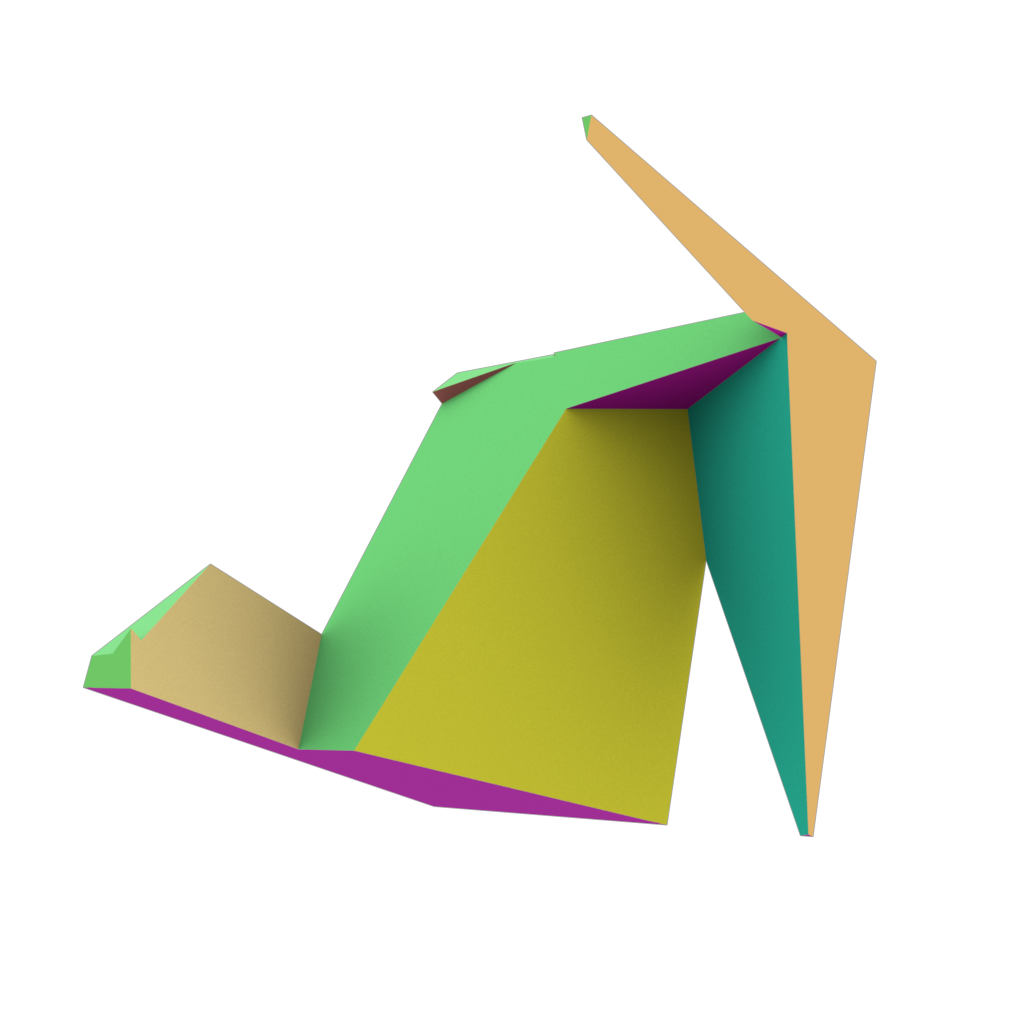
\includegraphics[width=0.24\textwidth]{images/0005.png}\hspace{-7mm}%
   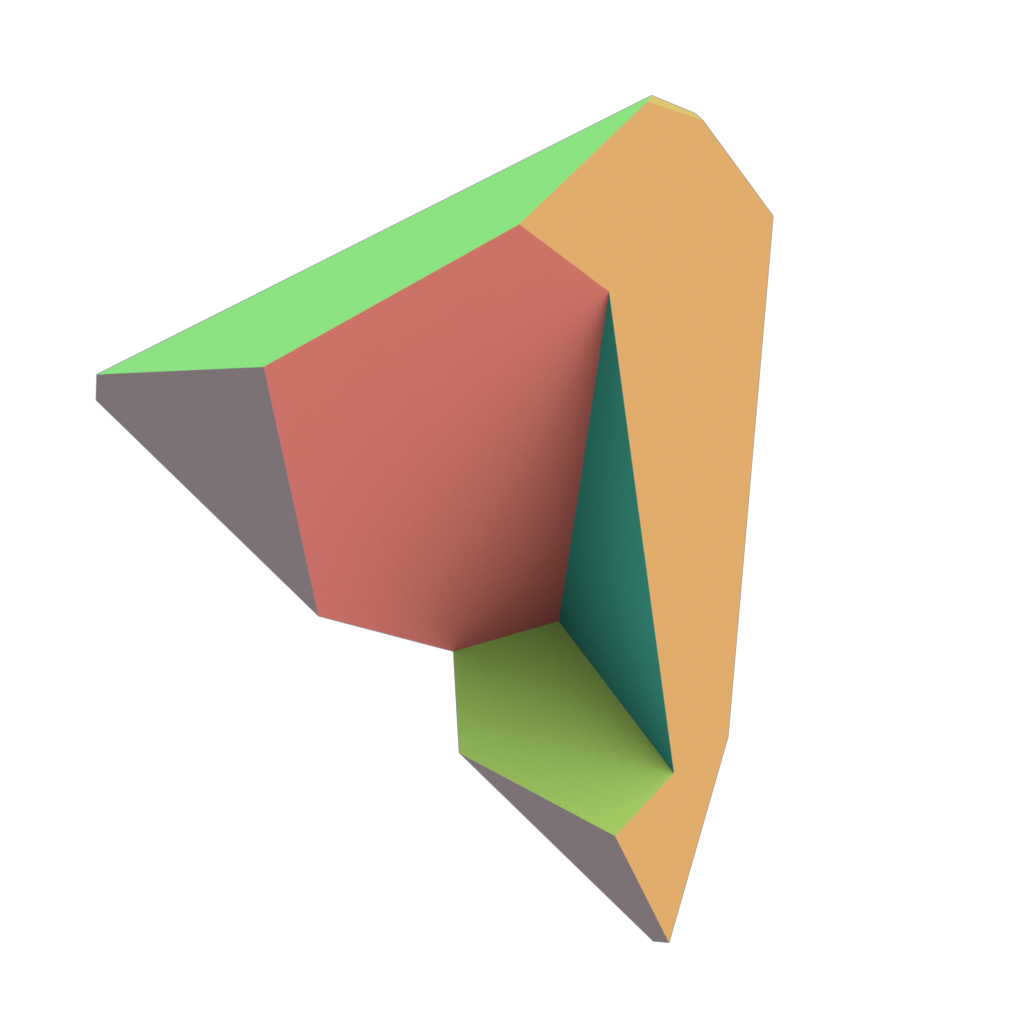
\includegraphics[width=0.22\textwidth]{images/0006.png}%
\vspace{-6mm}   
   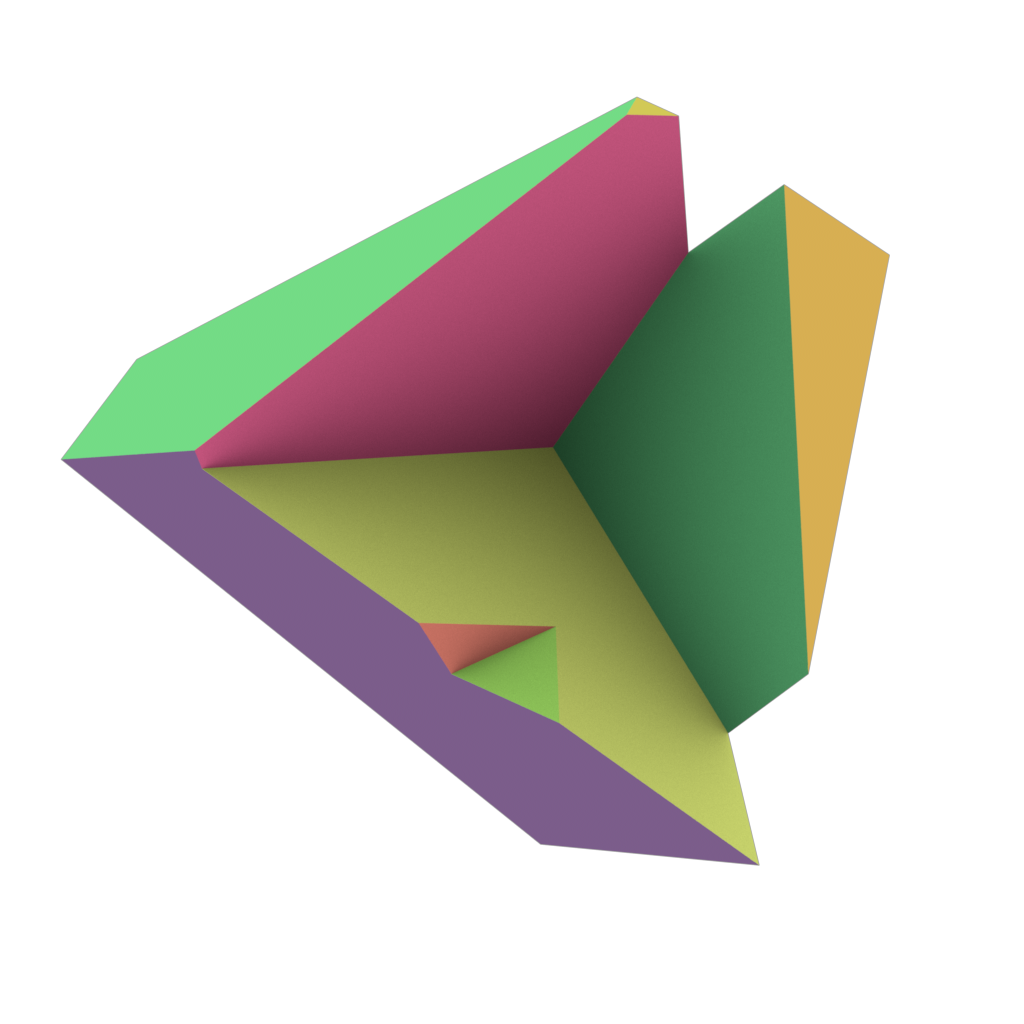
\includegraphics[width=0.25\textwidth]{images/0007.png}\hspace{-7mm}%
   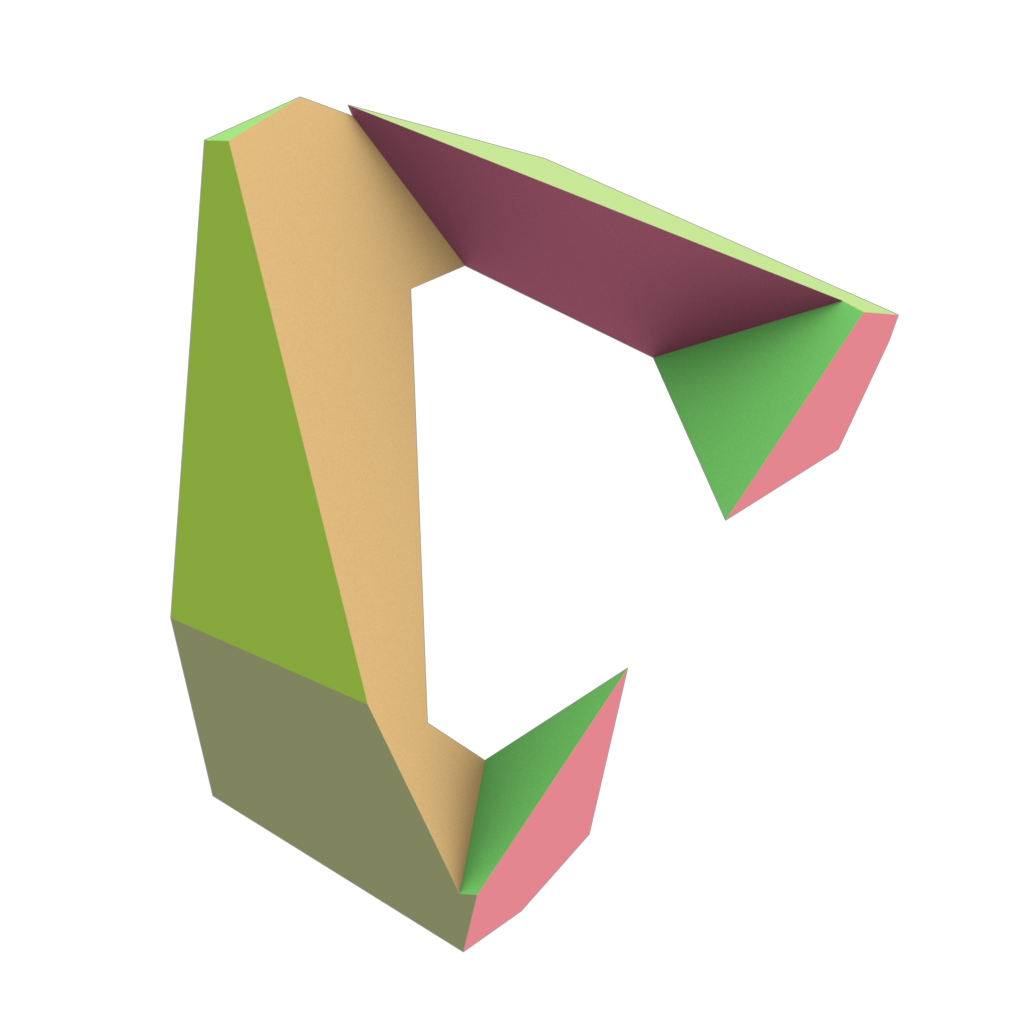
\includegraphics[width=0.23\textwidth]{images/0008.png}\hspace{-9mm}%
   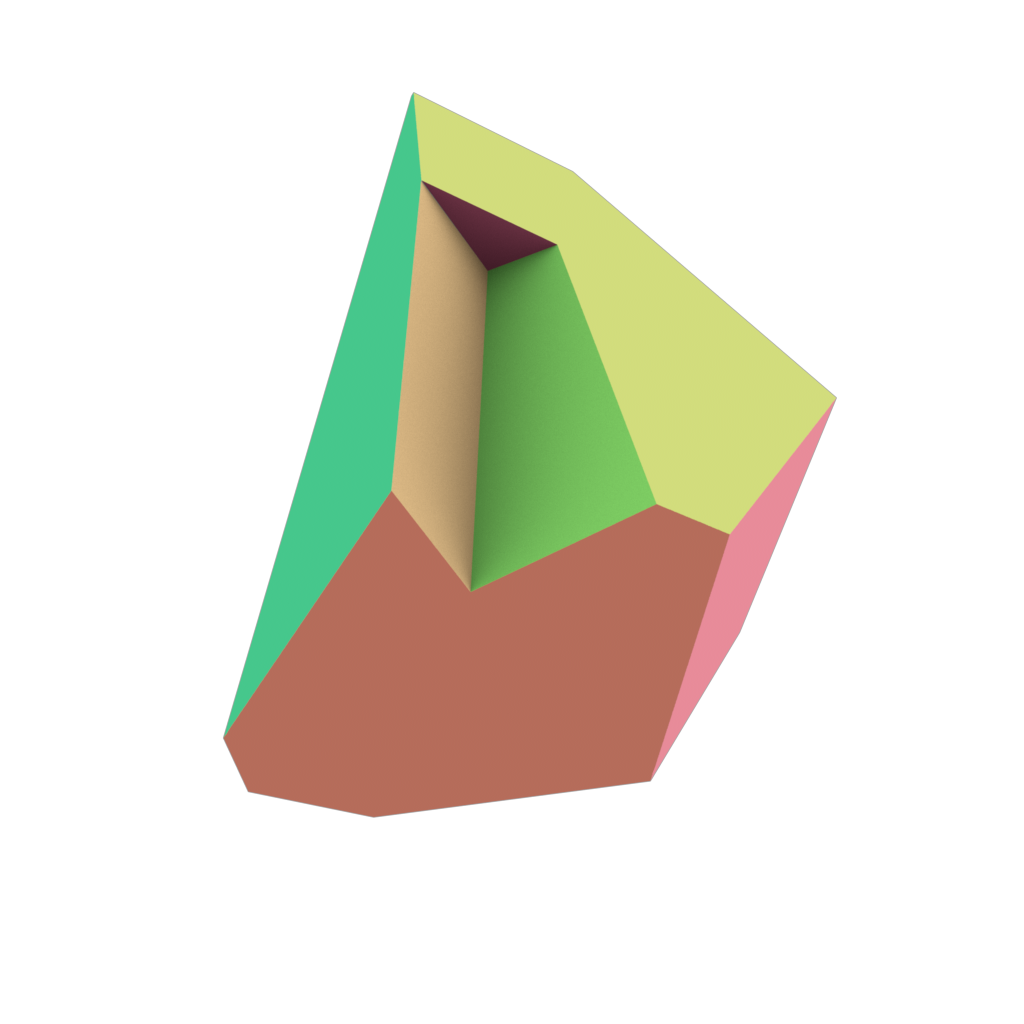
\includegraphics[width=0.25\textwidth]{images/0009.png}\hspace{-9mm}%
   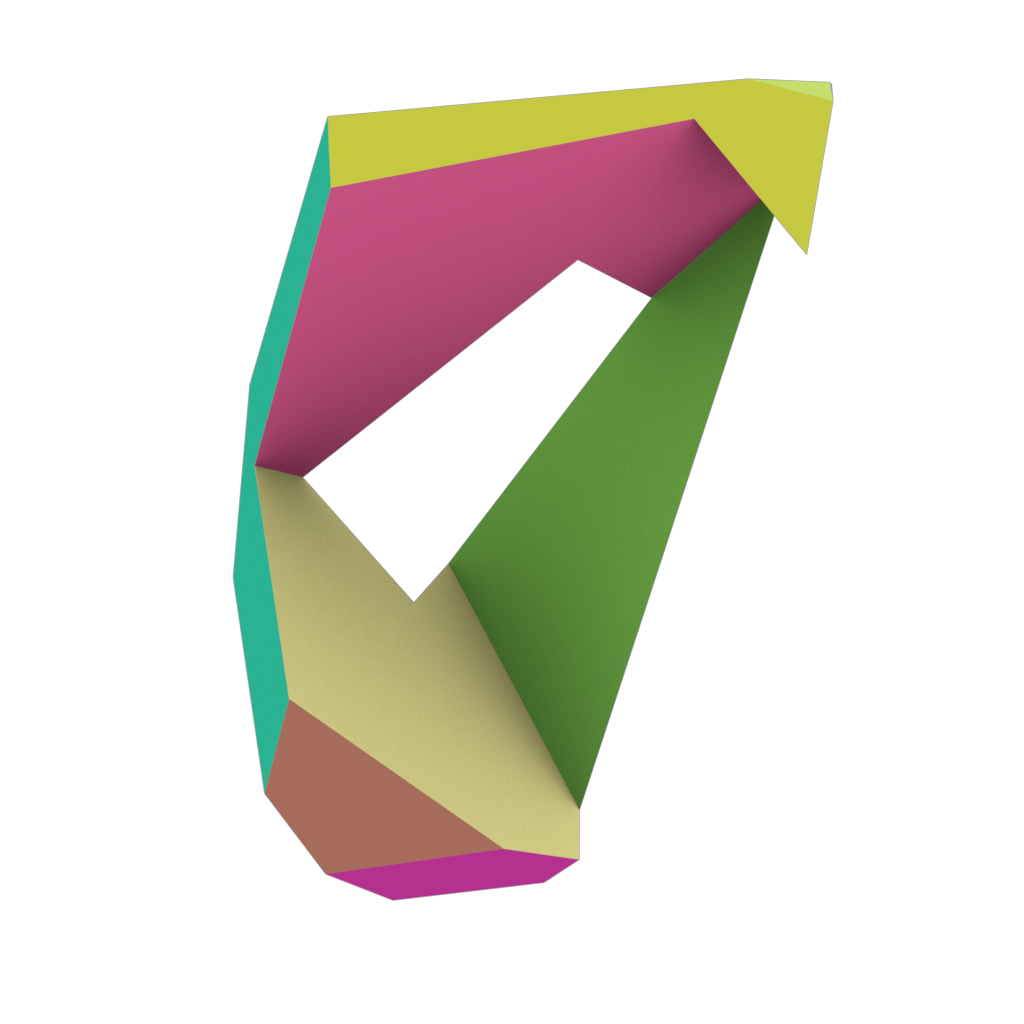
\includegraphics[width=0.23\textwidth]{images/0010.png}\hspace{-7mm}%
   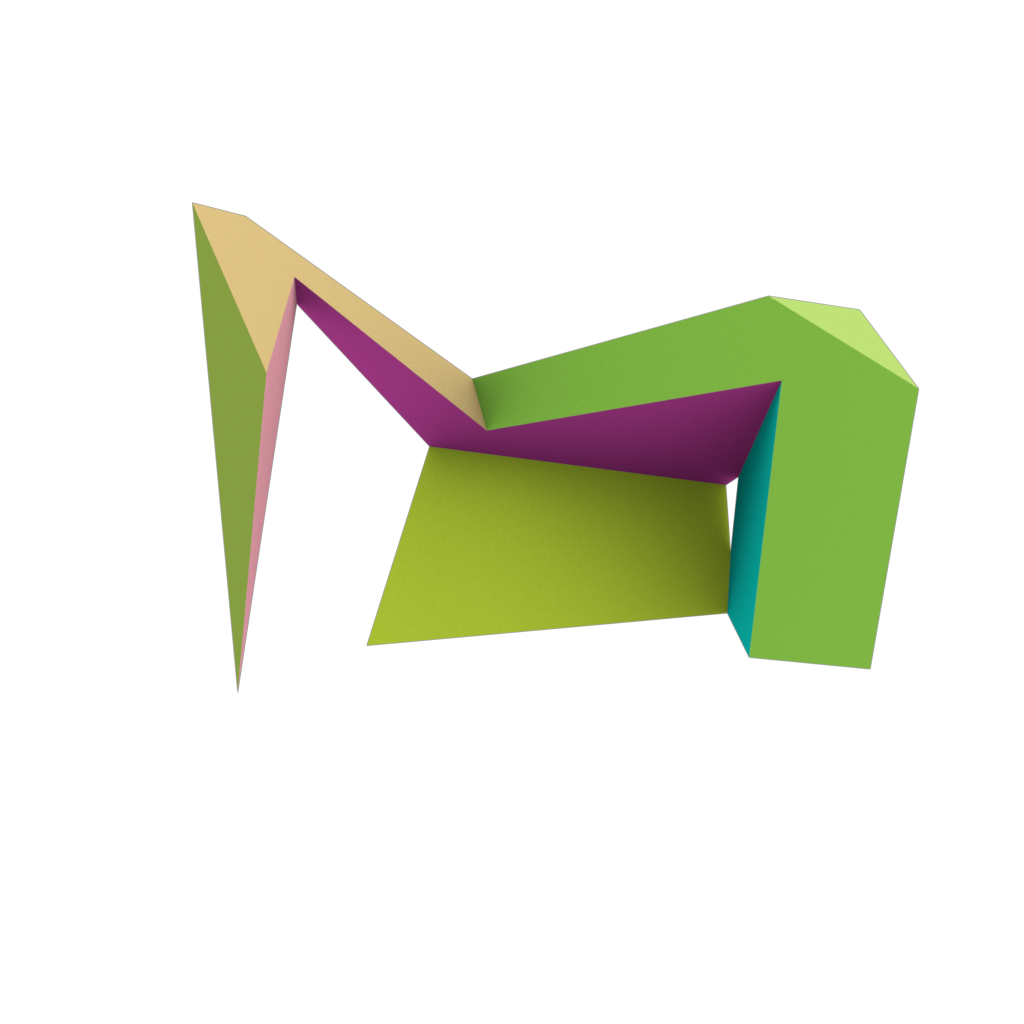
\includegraphics[width=0.25\textwidth]{images/0011.png}%
\vspace{-6mm}      
   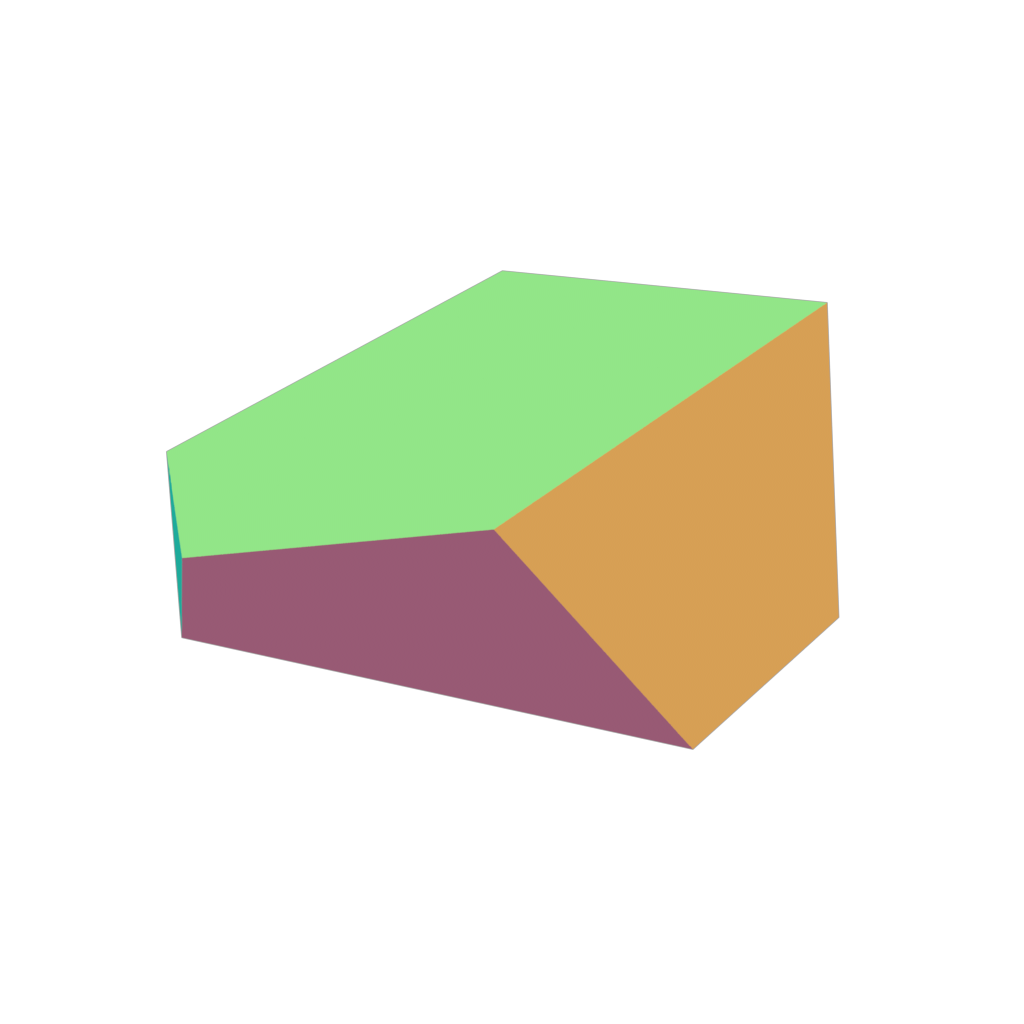
\includegraphics[width=0.20\textwidth]{images/0012.png}%
   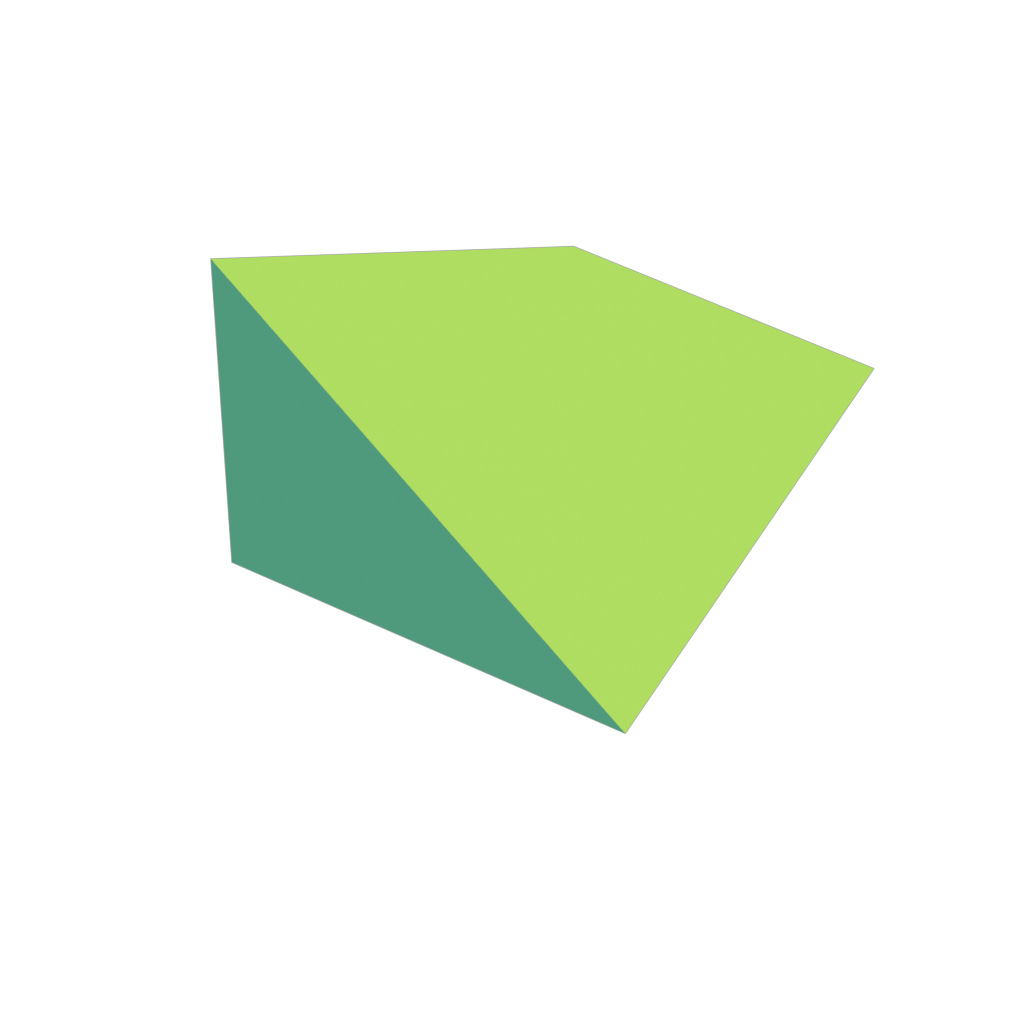
\includegraphics[width=0.20\textwidth]{images/0013.png}%
   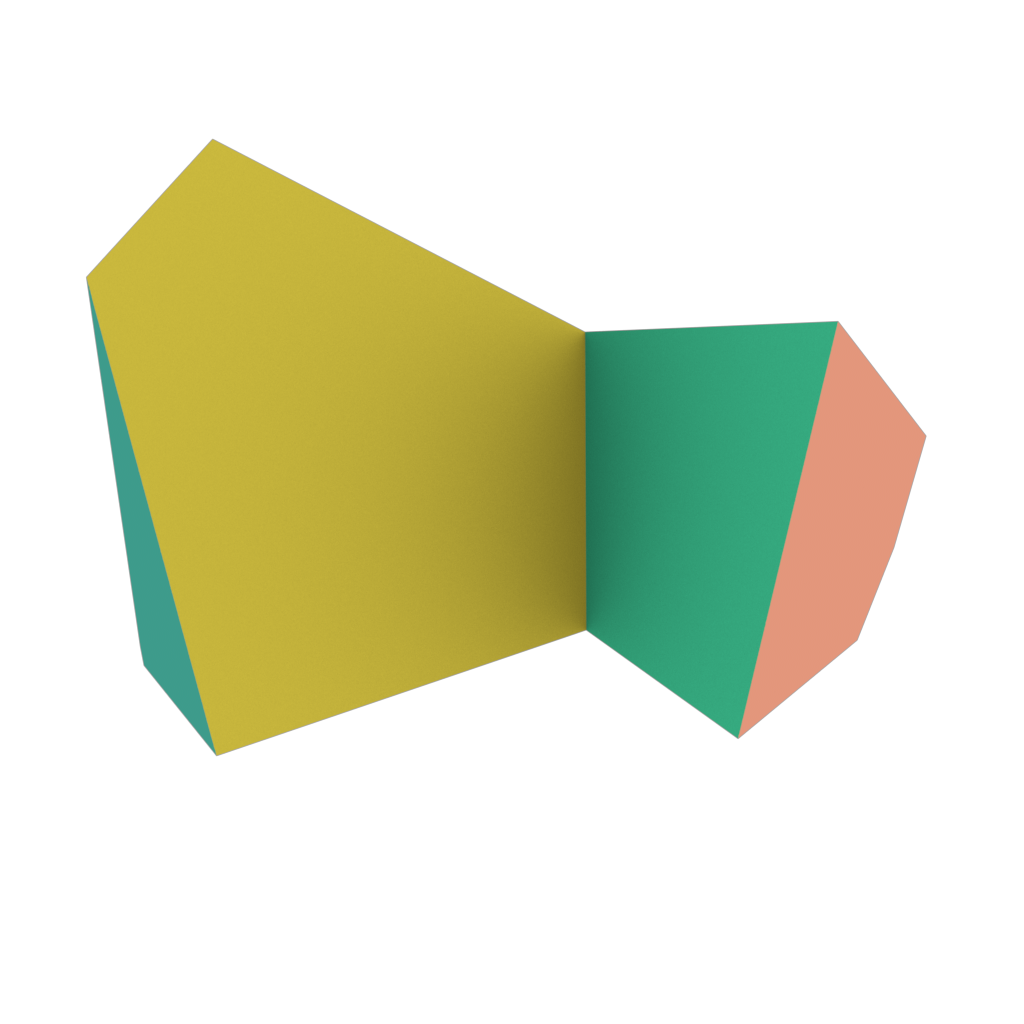
\includegraphics[width=0.20\textwidth]{images/0014.png}%
   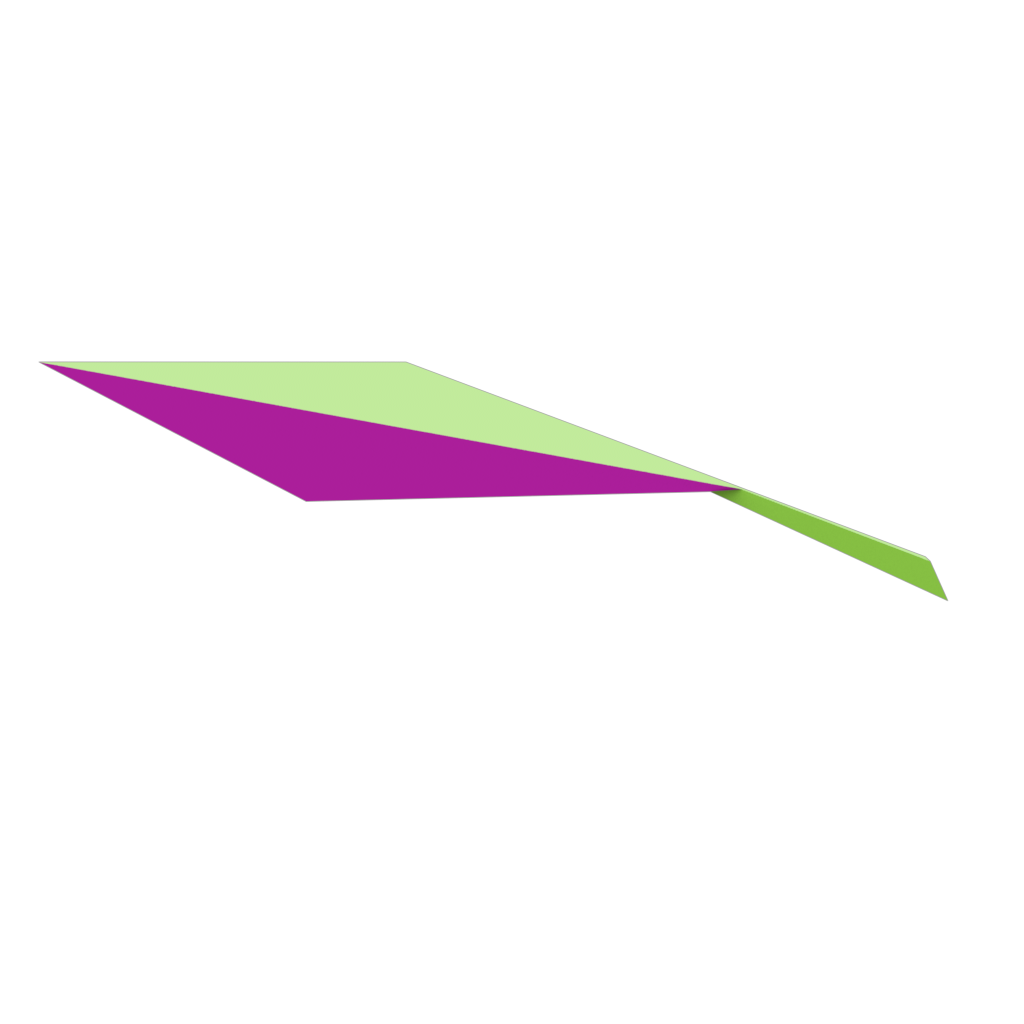
\includegraphics[width=0.20\textwidth]{images/0015.png}\hspace{-9mm}%
   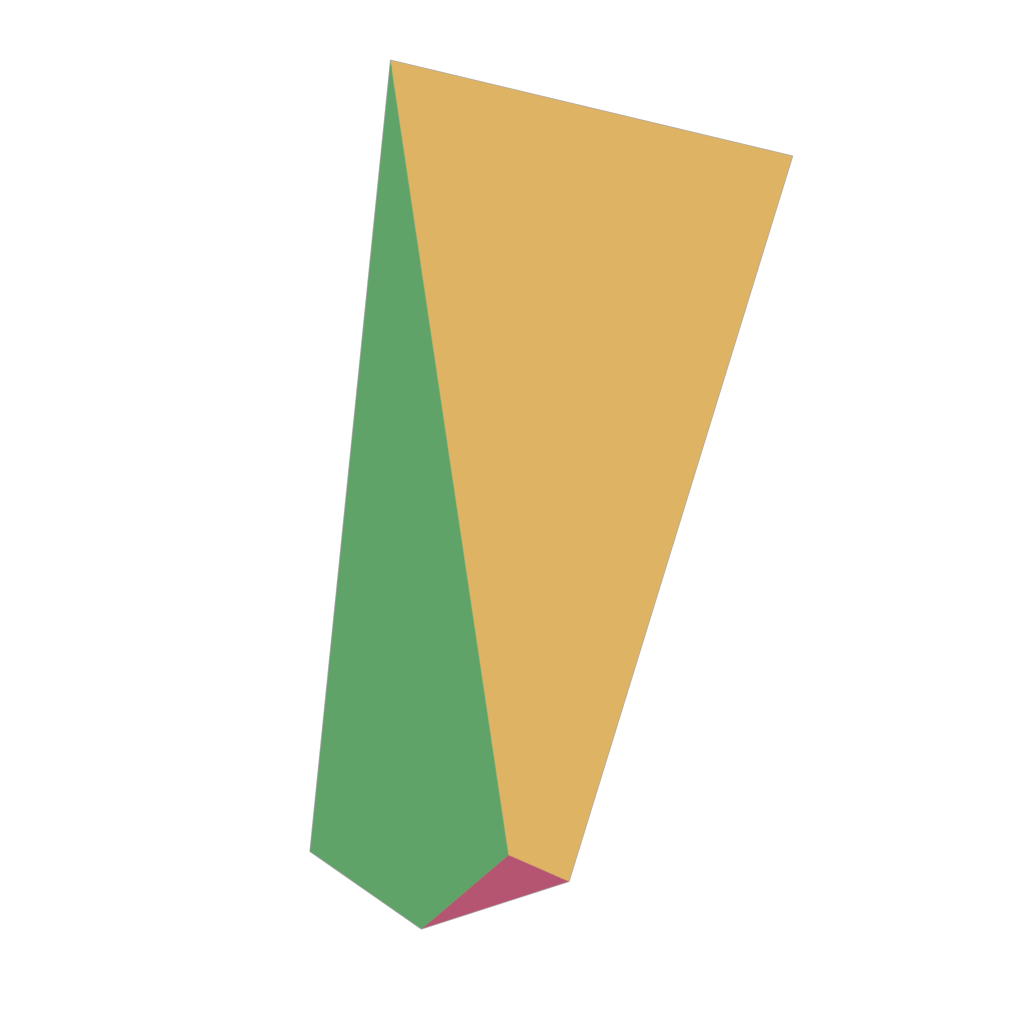
\includegraphics[width=0.20\textwidth]{images/0016.png}%
\vspace{-10mm}      
   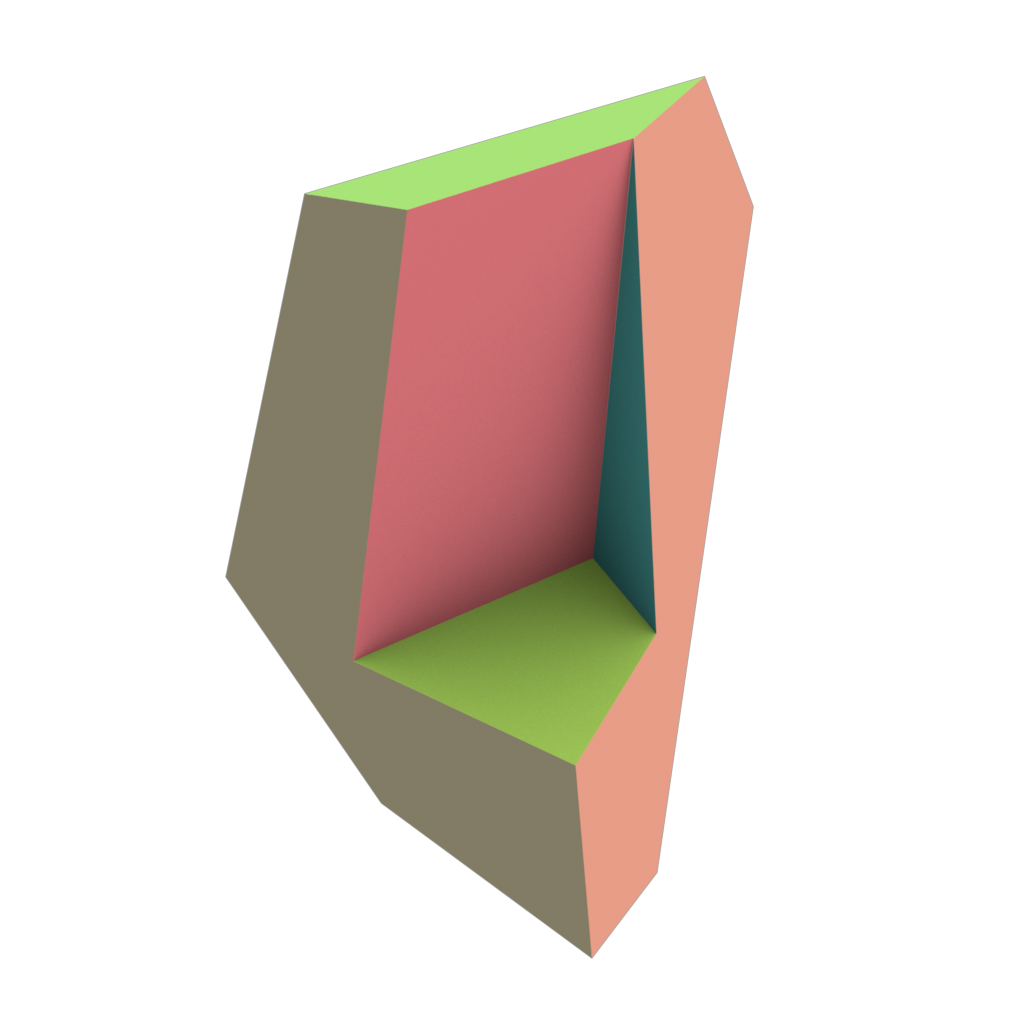
\includegraphics[width=0.20\textwidth]{images/0017.png}%
   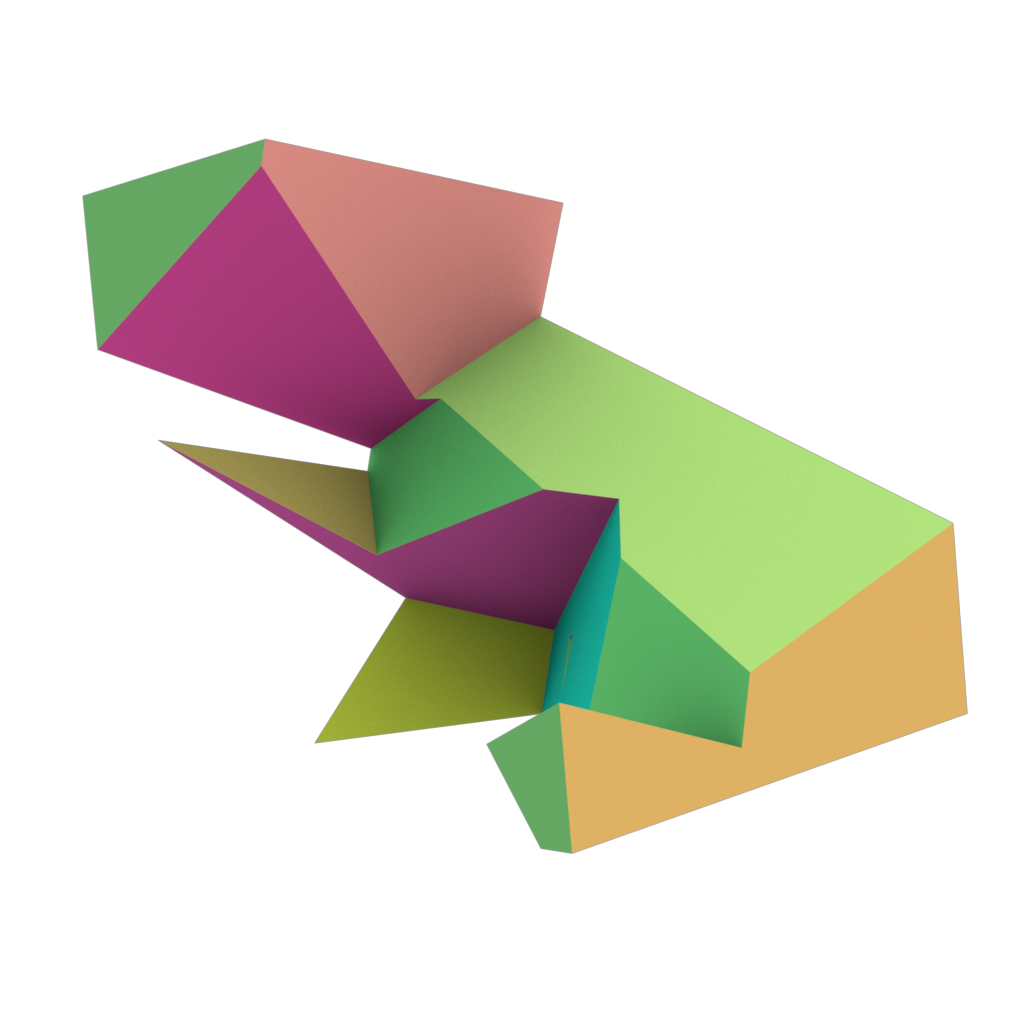
\includegraphics[width=0.25\textwidth]{images/0019.png}\hspace{-7mm}%
   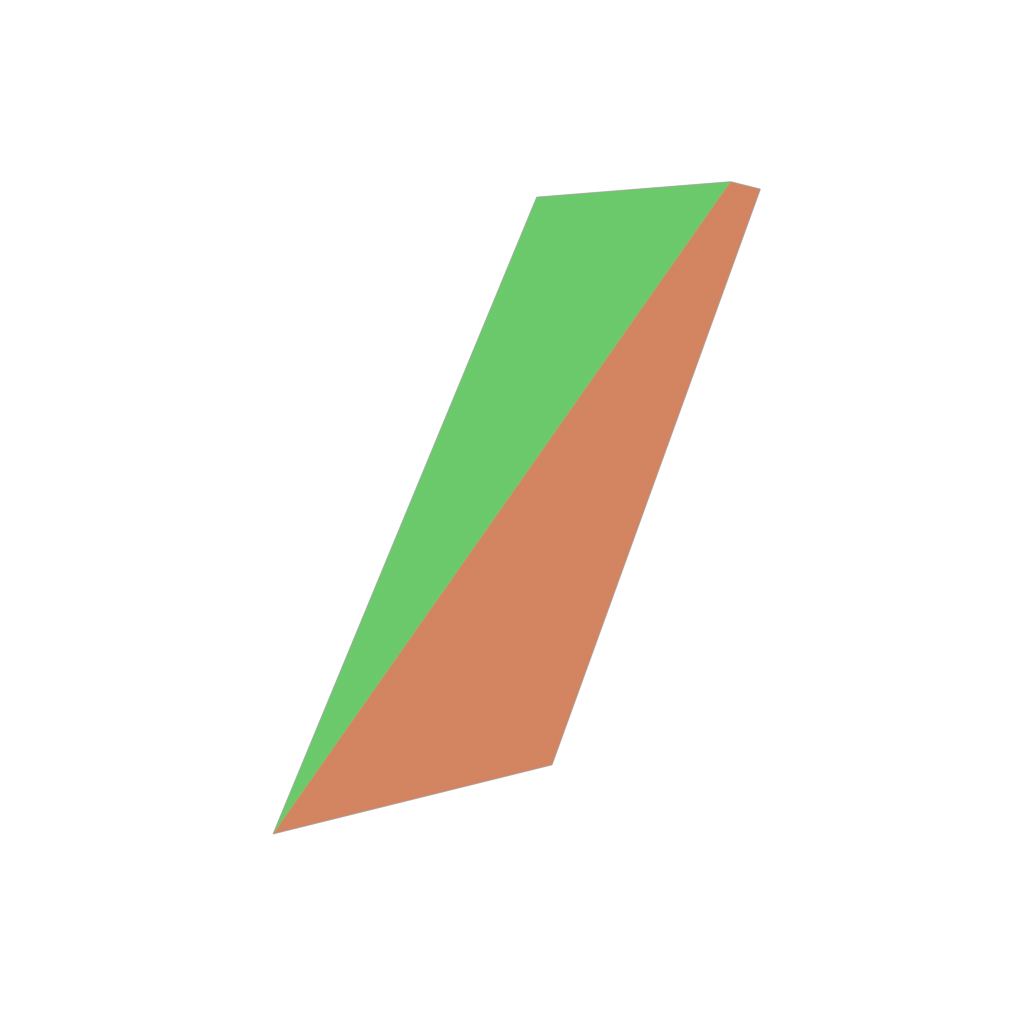
\includegraphics[width=0.20\textwidth]{images/0020.png}\hspace{-7mm}%
   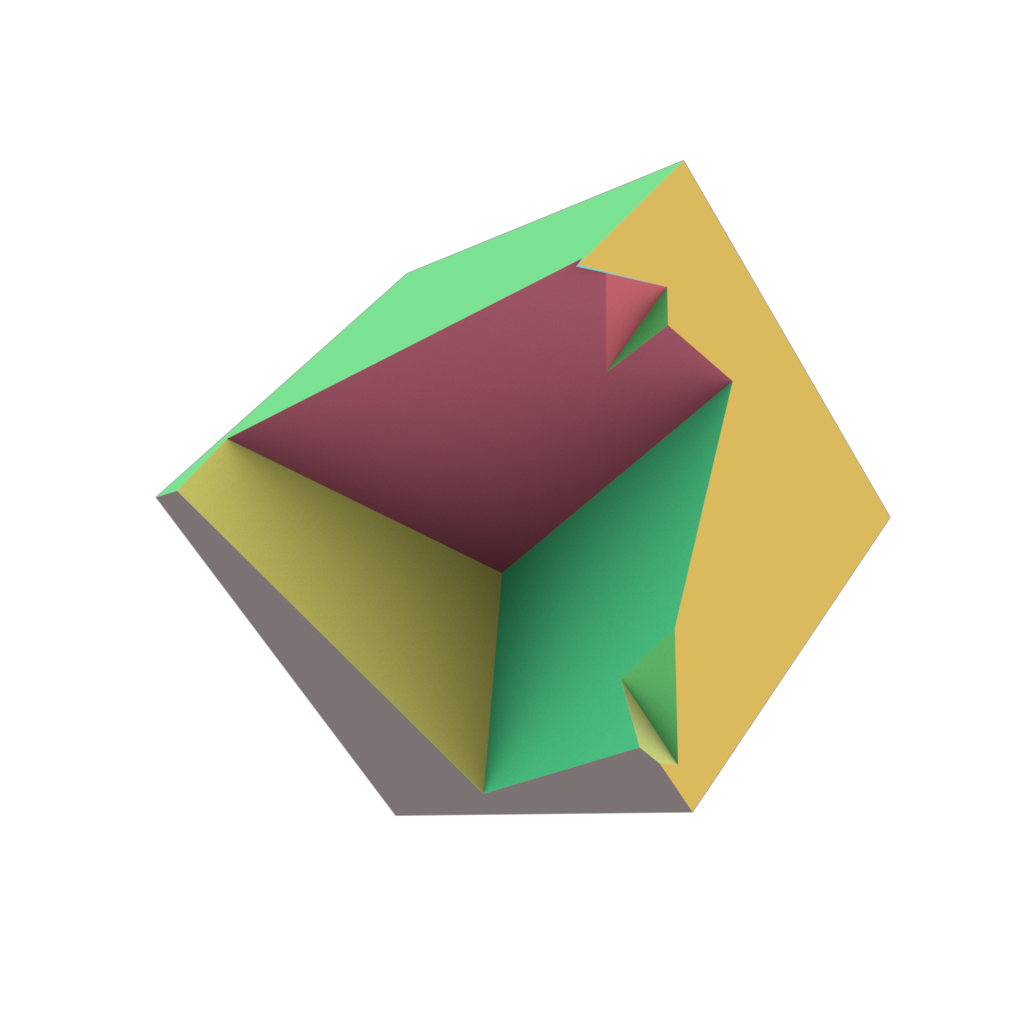
\includegraphics[width=0.25\textwidth]{images/0021.png}\hspace{-7mm}%
   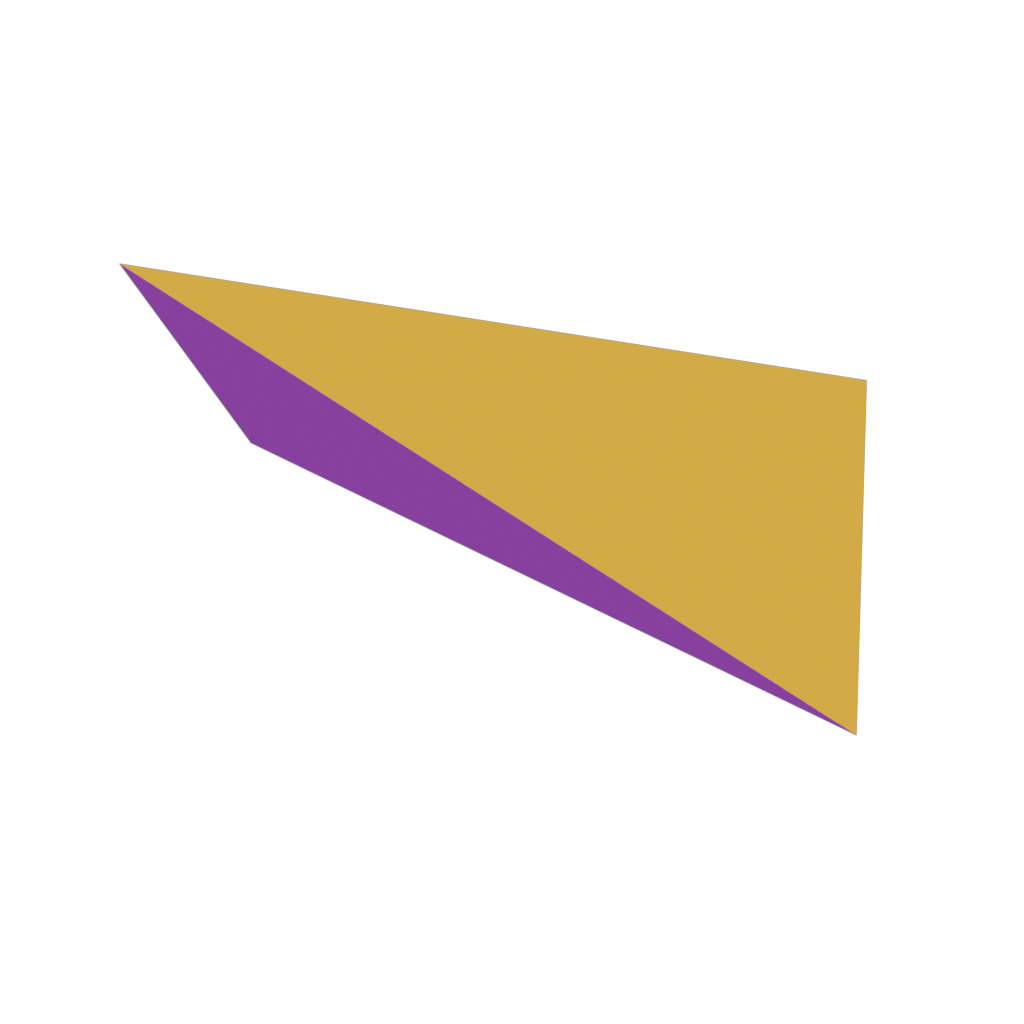
\includegraphics[width=0.20\textwidth]{images/0022.png}%
\vspace{-10mm}      
   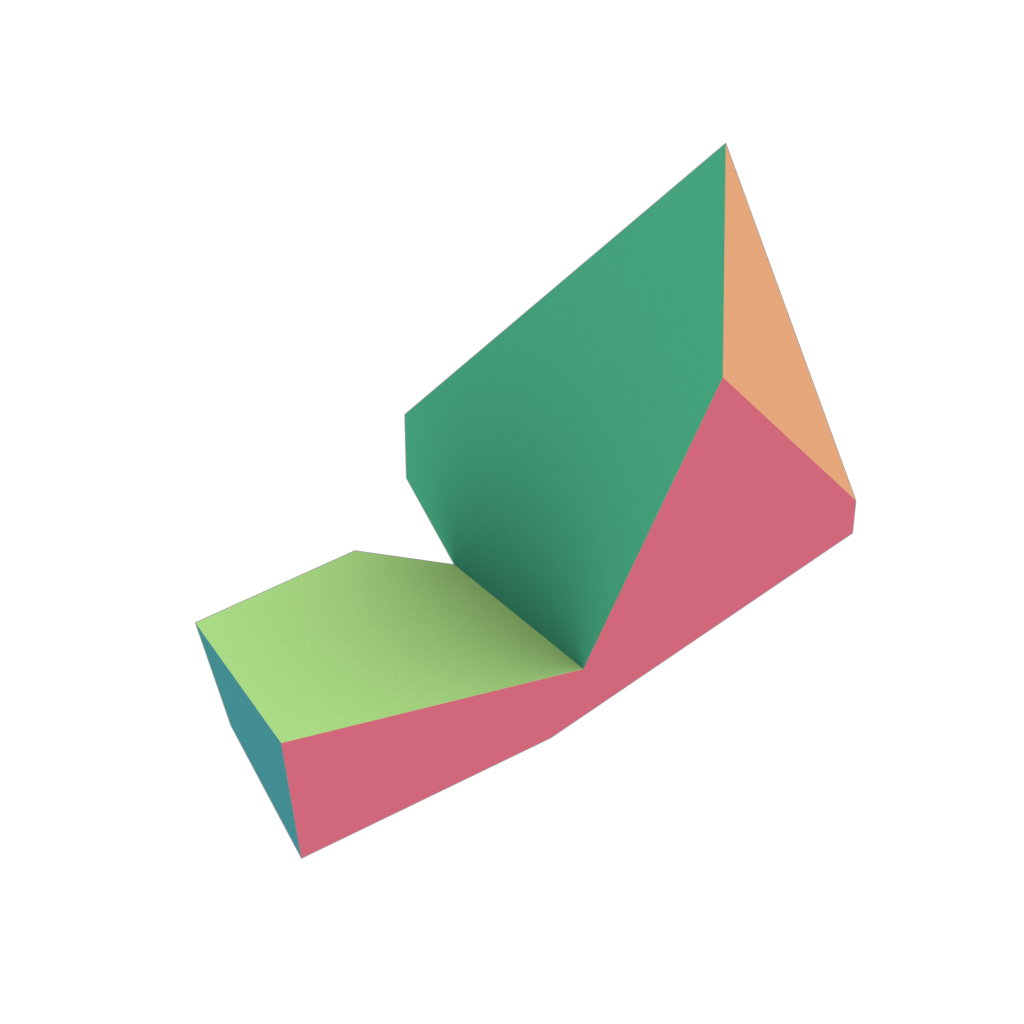
\includegraphics[width=0.20\textwidth]{images/0023.png}\hspace{3mm}%
   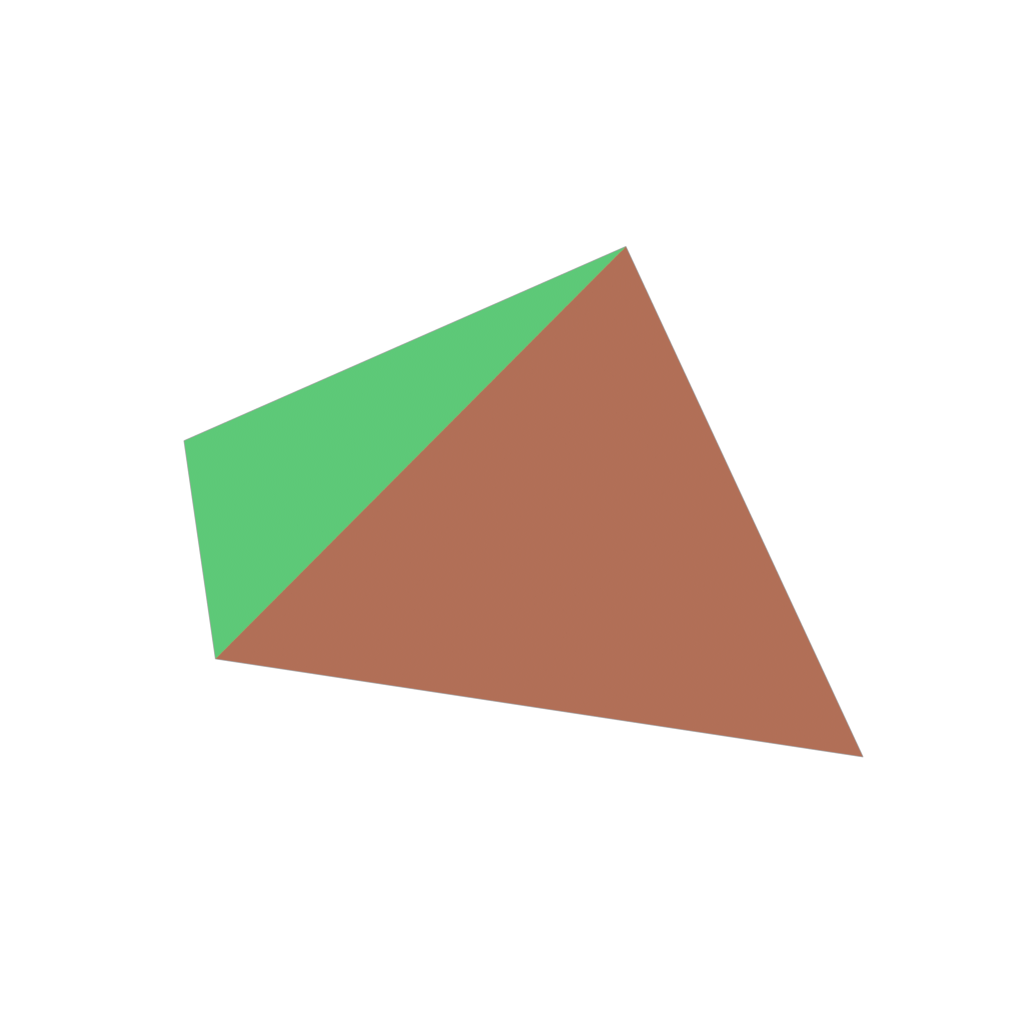
\includegraphics[width=0.18\textwidth]{images/0024.png}%
   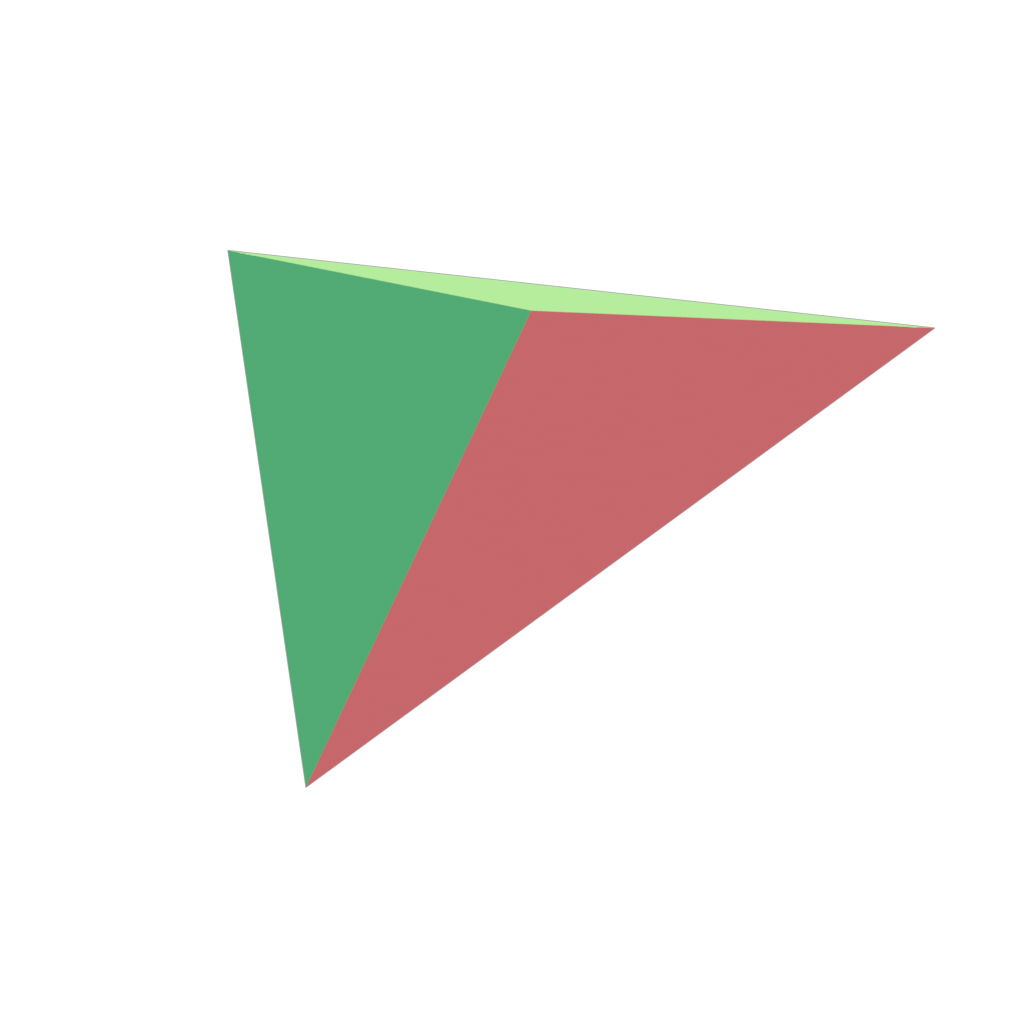
\includegraphics[width=0.18\textwidth]{images/0025.png}%
   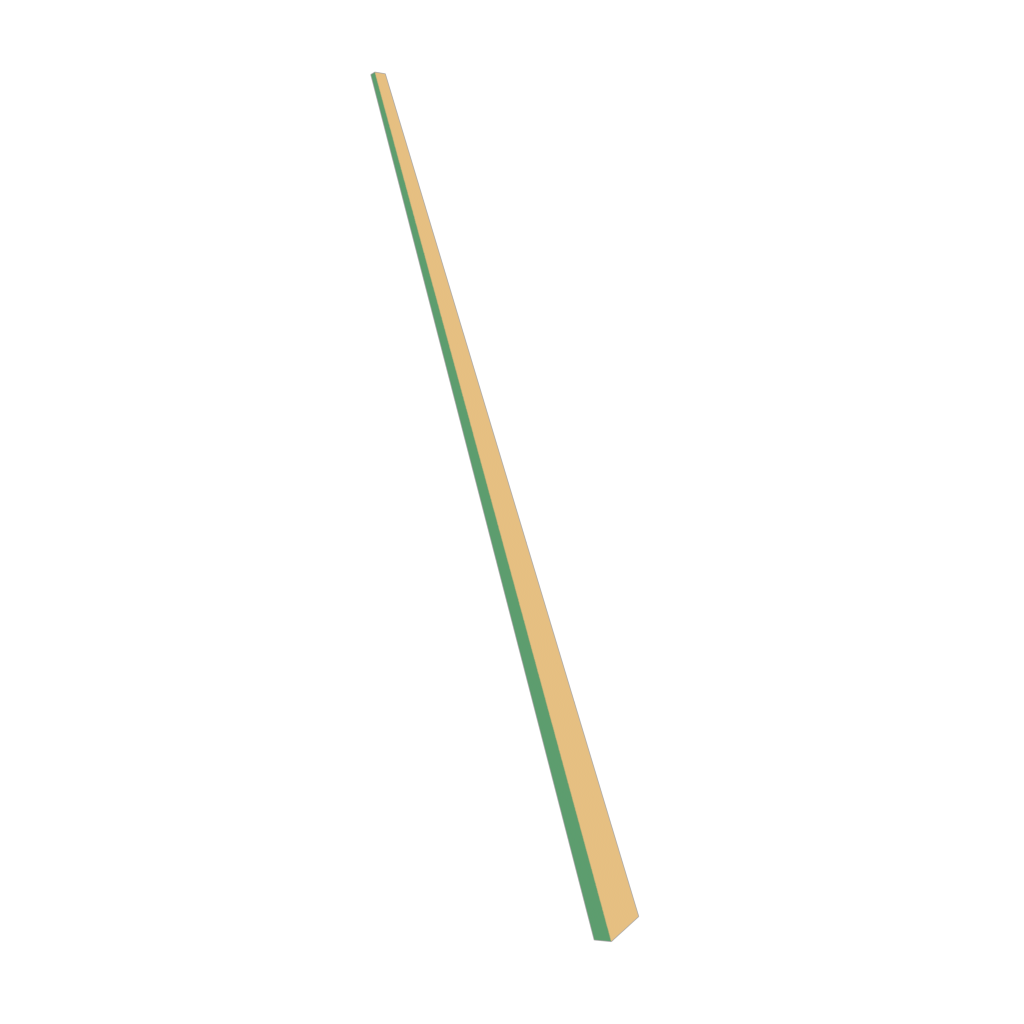
\includegraphics[width=0.15\textwidth]{images/0026.png}\hspace{-7mm}%
   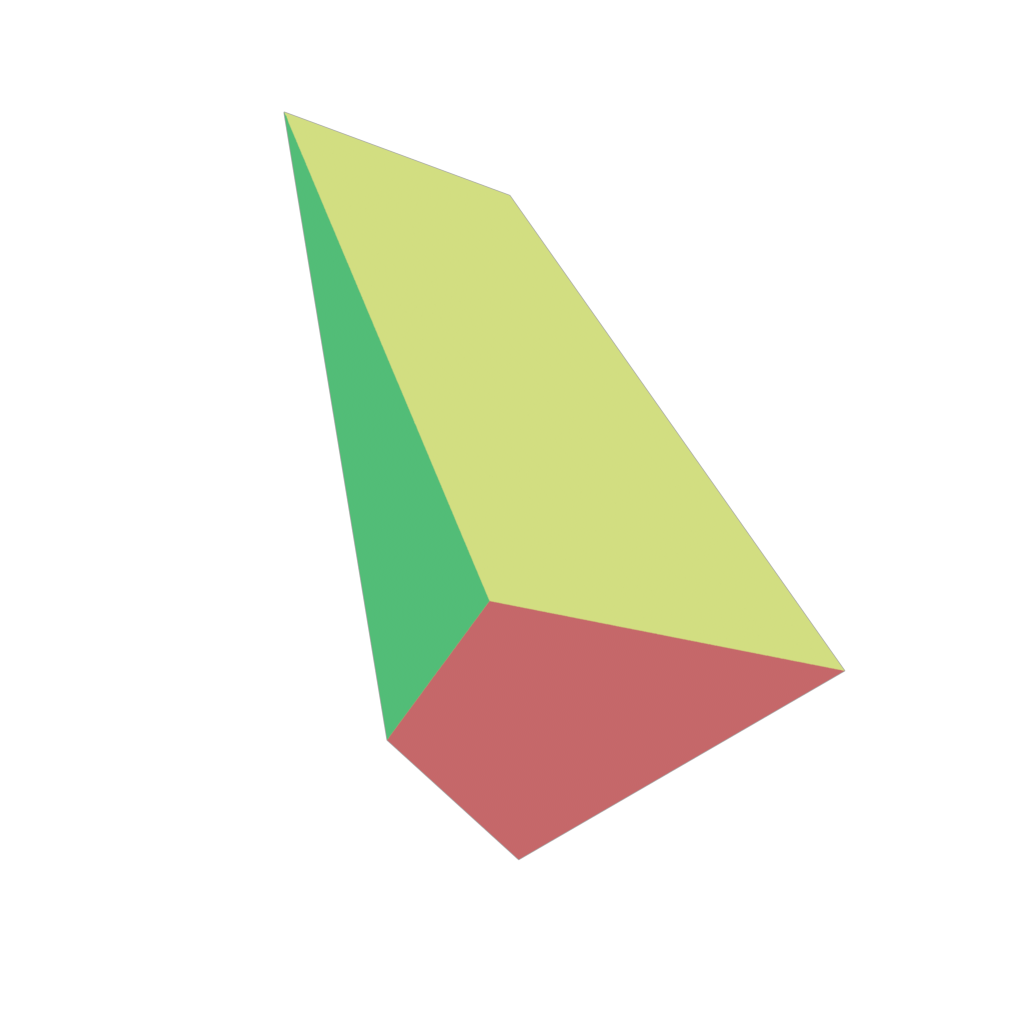
\includegraphics[width=0.20\textwidth]{images/0027.png}%
\caption{The 3-cells of the arrangement of $\E^3$ generated by our collection of five random cubes.
   The 3-cells are here not in scale, and suitably rotated to better show their complex structure.
   Their assembly provides the union of the five cubes.
   Each \emph{3-cell is given} by \emph{a column} of the \emph{sparse matrix} of \emph{chain map} $\delta_2: C_2\to C_3$, i.e.~by \texttt{copCF}, with values in $\{-1,0,1\}$.
   }
   \label{fig:3-cells}
\end{figure}
Look for this purpose at the fourth cell (from left) of the second row (from top) of Figure~\ref{fig:3-cells}. Other 3-cells have also smaller holes in the faces and/or tunnels within. The boundary triangulation of 3-cells  needed to generate graphics on a display device or for 3D printing is also provided in \href{https://github.com/cvdlab/LinearAlgebraicRepresentation.jl}{our package {repository} on \texttt{github.com}}.

The geometric model of the arrangement is generated as a pair (\emph{Geometry}, \emph{Topology}), where the first one is simply given by the embedding map \texttt{V} of vertices (0-cells), i.e. by their coordinate matrix, given by columns:

\vspace{1mm}
\noindent
{\small 
\begin{verbatim}
julia> V
3x137 Array{Float64,2}:
 1.01181   0.215639  0.516927  0.449016 ... 1.01221   1.30039   0.741732  1.02991
 0.160033  0.06801   0.102833  0.094984 ... 0.816151  0.545669  1.51776   1.24728
 0.196256  0.206963  0.202911  0.203825 ... 0.249344  0.985248  0.613139  1.34904
\end{verbatim}}
\vspace{1mm}

The cardinality of 0-, 1-, 2-, and 3-cell sets \texttt{V}, \texttt{E}, \texttt{F}, \texttt{C} are given as row and column numbers of the sparse matrices of their signed incidence relations \texttt{EV}, \texttt{FE}, \texttt{CF}, that can be interpreted as coboundary operators $\delta_0$ (from vertices to edges), $\delta_1$ (from edges to faces), and $\delta_2$ (from faces to solid cells), respectively. The prefix \texttt{cop} stands for \emph{chain operator}:

\vspace{3mm}
\noindent
\begin{minipage}[l]{.333\textwidth}
{\small \begin{verbatim}
julia> copEV
268x137 SparseMatrixCSC
with 536 stored entries:
  [1  ,   1]  =  -1
  [5  ,   1]  =  -1
  [39 ,   1]  =  -1
  ...
  [258, 137]  =  1
  [260, 137]  =  1
  [268, 137]  =  1
\end{verbatim}}
\end{minipage}% 
\hfill
\begin{minipage}{.333\textwidth}
{\small \begin{verbatim}
julia> copFE
157x��268 SparseMatrixCSC
with 786 stored entries:
  [1  ,   1]  =  1
  [11 ,   1]  =  1
  [2  ,   2]  =  1
  ...
  [156, 267]  =  1
  [150, 268]  =  1
  [157, 268]  =  1
\end{verbatim}}
\end{minipage}% 
\hfill
\begin{minipage}{.333\textwidth}
{\small \begin{verbatim}
julia> copCF
27x157 SparseMatrixCSC 
with 314 stored entries:
  [1  ,   1]  =  -1
  [19 ,   1]  =  1
  [2  ,   2]  =  -1
  ...
  [21 , 156]  =  1
  [1  , 157]  =  1
  [21 , 157]  =  -1
\end{verbatim}}
\end{minipage}% 
\vspace{1mm}


\subsection{The input collection of surfaces}
%-------------------------------------------------------------------------------
The input data for the example of Figure~\ref{fig:input} was generated by a little script in Julia language, which is not of interest here. Conversely, we provide below the full input, i.e.~both the geometry \texttt{V} and the topology \texttt{EV, FV}. Such text data amount to 2.1$k$ bytes. 

\vspace{1mm}
\noindent
{\footnotesize
\begin{verbatim}
julia> @show V; 
V = [1.01181 0.215639 0.91979 0.123616 1.02252 0.226347 0.930498 0.134324 0.0458309 
-0.301827 0.348275 0.0006172 0.579367 0.23171 0.881811 0.534154 -0.0521776 0.627953 
-0.190635 0.489496 -0.0233884 0.656742 -0.161846 0.518285 0.27652 -0.0875132 0.52527 
0.161237 0.509324 0.145291 0.758074 0.394041 0.27631 0.564484 0.0058279 0.294002 
1.01221 1.30039 0.741732 1.02991; 0.160033 0.0680099 0.956278 0.864255 0.160649 
0.0686266 0.956895 0.864872 -0.200245 0.102199 0.417839 0.720283 -0.35354 -0.0510965 
0.264543 0.566987 0.682359 0.543901 0.0592036 -0.0792537 0.956374 0.817917 0.333219 
0.194762 -0.102028 0.146722 0.324834 0.573584 -0.16916 0.0795901 0.257702 0.506452 
0.452356 0.181874 1.15396 0.883481 0.816151 0.545669 1.51776 1.24728; 0.196256 0.206963 
0.196872 0.20758 0.997729 1.00844 0.998346 1.00905 0.0677451 0.601282 -0.0855504 
0.447986 0.502301 1.03584 0.349005 0.882542 0.159301 0.18809 0.433316 0.462105 0.797002 
0.825792 1.07102 1.09981 0.1446 0.377404 0.0774682 0.310272 0.580364 0.813168 0.513232 
0.746036 0.403805 1.13971 0.767599 1.5035 0.249344 0.985248 0.613139 1.34904]
\end{verbatim}}

{\footnotesize
\begin{verbatim}
julia> @show FV,EV;
(FV,EV) = (Array{Int64,1}[[1,2,3,4],[5,6,7,8],[1,2,5,6],[3,4,7,8],[1,3,5,7],[2,4,6,8],
[9,10,11,12],[13,14,15,16],[9,10,13,14],[11,12,15,16],[9,11,13,15],[10,12,14,16],[17,
18,19,20],[21,22,23,24],[17,18,21,22],[19,20,23,24],[17,19,21,23],[18,20,22,24],[25,26,
27,28],[29,30,31,32],[25,26,29,30],[27,28,31,32],[25,27,29,31],[26,28,30,32],[33,34,35,
36],[37,38,39,40],[33,34,37,38],[35,36,39,40],[33,35,37,39],[34,36,38,40]], 
Array{Int64,1}[[1,2],[3,4],[5,6],[7,8],[1,3],[2,4],[5,7],[6,8],[1,5],[2,6],[3,7],[4,8],
[9,10],[11,12],[13,14],[15,16],[9,11],[10,12],[13,15],[14,16],[9,13],[10,14],[11,15],
[12,16],[17,18],[19,20],[21,22],[23,24],[17,19],[18,20],[21,23],[22,24],[17,21],[18,
22],[19,23],[20,24],[25,26],[27,28],[29,30],[31,32],[25,27],[26,28],[29,31],[30,32],
[25,29],[26,30],[27,31],[28,32],[33,34],[35,36],[37,38],[39,40],[33,35],[34,36],[37,
39],[38,40],[33,37],[34,38],[35,39],[36,40]])
\end{verbatim}}

\subsection{The generating script}
%-------------------------------------------------------------------------------
Below we  compute the cellular 3-complex of the $\E^3$ space partition induced by the above collection of surfaces.
In the current prototype implementation, some transformation of input data format is needed. A simpler  API will be provided soon. In particular, type \texttt{Lar.Cells} (array of arrays of integers) is converted to type \texttt{Lar.ChainOp}, i.e., the Julia's type \texttt{SparseMatrixCSC\{Int8,Int64\}} for  sparse matrices.

\vspace{2mm}
{\small
\begin{verbatim}
Lar = LinearAlgebraicRepresentation

cop_EV = Lar.coboundary_0(EV::Lar.Cells);
cop_EW = convert(Lar.ChainOp, cop_EV);
cop_FE = Lar.coboundary_1(V, FV::Lar.Cells, EV::Lar.Cells);
W = convert(Lar.Points, V');

V, copEV, copFE, copCF = Lar.Arrangement.spatial_arrangement(
                         W::Lar.Points, cop_EW::Lar.ChainOp, cop_FE::Lar.ChainOp )
\end{verbatim}}
\vspace{2mm}



\subsection{The output chain complex}
%-------------------------------------------------------------------------------


It is easier to compare different data structures by their number of data objects and/or textual file size, without taking into account the actual computational architecture and the memory occupancy.

Therefore, some comparison numbers follow: into the five (unconnected) boundaries of our input \texttt{Lar} cubes there are $5\times 8=40$ vertices, $5\times 6=30$ quads, and $5\times 12=60$ edges. For the computed space arrangement, 137 vertices and 953 triangles are contained within the 27 cell groups of the output \texttt{OBJ} file. The arrays of vertices, edges, faces and 3-cells, without any added data structure\footnote{The incidence relations are computable on demand by product or transposition of sparse binary \emph{characteristic matrices}, as discussed in Reference~\cite{TSAS}}, are given in Ref.\footnote{{\scriptsize
\texttt{\href{https://github.com/cvdlab/LinearAlgebraicRepresentation.jl/tree/julia-1.1/examples/3d/data}{https://github.com/cvdlab/LinearAlgebraicRepresentation.jl/tree/julia-1.1/examples/3d/data}},
}
} and weight for 38 kB as text file.

The cellular 3-complex output with 
137 0-cells, 268 1-cells, 157 2-cells, 27 3-cells, for a total of $589$ graded $p$-cells, is better represented as a (geometric) \emph{chain complex}. In particular, 
the textual values of \texttt{V}, together with sparse matrices \texttt{copEV} and \texttt{copFE}, computed by the  \emph{Merge} algorithm~\cite{TSAS}, plus the sparse matrix \texttt{copCF} computed by the \emph{TGW} algorithm~\cite{TSAS} in 3D, are given in \texttt{\href{https://github.com/cvdlab/LinearAlgebraicRepresentation.jl}{github.com/}}\footnote{\emph{idem}}
for a file size of (4+12+2)$k$ bytes. 

It migth be interesting to note that the minimal and fairly crude \texttt{\texttt{OBJ}} file representation of 3-cells, also provided in \footnote{\emph{idem}}, amounts to (4+11)$k$ bytes.  But whereas this last format just contains a bunch of triangles as triples of indices of vertices, without any storage of the assembly and cells topology, the \emph{chain complex} representation conversely provides a complete understanding of topology and either single or multiple querying of topological features, using only sparse matrix-vector or sparse matrix-matrix  multiplications, respectively. 


%===============================================================================
\section{Conclusion}
%===============================================================================

In this short \emph{Addendum} to \emph{Topological Computing of Arrangements with (Co)chains}, a small example of computation of a 3D arrangement has been presented and discussed. The main aim was to show the fairly general nature of generated 3-cells, that are connected and non manifold, non  contractible, and with any topological genus. We would like to remark also the briefness and simplicity  of this representation of \emph{geometric models} as \emph{chain complexes}, and its great generality. 
The authors hope that the presented material may help to better understand such a novel approach to geometric computing using algebraic topological tools. 


% Bibliography
\bibliographystyle{amsplain}
\bibliography{TSAS-2019.bib}


\end{document}  